%% This is an example first chapter.  You should put chapter/appendix that you
%% write into a separate file, and add a line \include{yourfilename} to
%% main.tex, where `yourfilename.tex' is the name of the chapter/appendix file.
%% You can process specific files by typing their names in at the 
%% \files=
%% prompt when you run the file main.tex through LaTeX.
\chapter{Data Analysis}

\section{Analysis Tools}

In this thesis, the analysis tools we use is based on Macbook computers, and CMS high computing, linux shell script, C++ programing language, and ROOT analysis package for high energy physics experiments. The machine performing the analysis includes CERN lxplus, MIT Tier-2 submit, Data file are saved as ROOT files format. Data samples are processed with crab CERN lxplus and MIT submit condor job submission with parallel computing framework. The core software for the data process and analysis is the CMS software (CMSSW\_10\_3\_4). The codes for the analysis software is documented on github and gitlab. Throughout the analysis, we use Poison statistics to interpret the statistical uncertainties of the data. In the limit of high statistics, it is approximately equivalent to Gaussian Statistics. In the limit of low statistics, it is different from Gaussian Statistics. These tools are crucial for me to finish the analysis and present the results.

\section{Analysis Strategies}

\subsection{Physics Goals}

The exclusive productions of b hadrons in different collision systems are necessary to study beauty energy loss and hadronization mechanisms. In this thesis, we propose to fully reconstruct $B^0_s$ and $B^+$ mesons in pp and PbPb collisions at $\sqrt{s_{NN}} = $ 5.02 TeV with the CMS experiment. We aim at measuring precisely their cross section, yield ratios, and nuclear modification factor of fully reconstructed $B^0_s$ and $B^+$ mesons via the decay channels of  to investigate beauty quark production and hadronization in vacuum and QGP. We hope to have a conclusive measurement of $B^0_s/B^+$ ratio to pinpoint the effect of strangeness enhancement in QGP on beauty hadronization and test theoretical model calculations \cite{StrangetoLight} with both fragmentation \cite{} and quark coalescence \cite{} mechanisms. Therefore, we would like to present our experimental measure over a width range of $p_T$ and centrality. We are particularly interested in the very low $p_T$ region where the slow moving beauty quark will pick up the nearby light quarks in the QGP while such mechanism is not expected to occur in the vacuum \cite{}. The $R_{AA}$ down to low $p_T$ will constrain understand beauty quark energy mechanism in the QGP medium. These will studies will be crucial for us to understand beauty quark diffusion coefficient and probe the inner workings of QGP in order to provide insights with the one of the open question in high energy nuclear physics.

\subsection{General Workflow}

Figure \ref{BsBPWorkFlow} shows workflow we designed to fully reconstructed $B^0_s$ and $B^+$ mesons from final state particles via the exclusive decay modes. The $B^0_s$ is fully reconstructed from the decay channel of $B^0_s \rightarrow J/\psi \phi \rightarrow \mu^+\mu^- K^+K^-$, which has a fragmentation fraction of $f(b\rightarrow B_s^0) =$ 0.103 and a decay branching fraction $BR(B^0_s \rightarrow J/\psi \phi \rightarrow \mu^+\mu^- K^+K^-) = 3.17 \times 10^{-5}$ $B^+ \rightarrow J/\psi K^+\rightarrow \mu^+\mu^- K^+$ with the CMS detector. The $B^+$ is fully reconstructed from the decay channel of $B^+ \rightarrow J/\psi \phi \rightarrow \mu^+\mu^- K^+$, which has a fragmentation fraction of $f(b\rightarrow B^+) =$ 0.401 and a decay branching fraction $BR(B^+ \rightarrow J/\psi \phi \rightarrow \mu^+\mu^- K^+K^-) = 6.02 \times 10^{-5}$ $B^+ \rightarrow J/\psi K^+\rightarrow \mu^+\mu^- K^+$ with the CMS detector. 



\begin{figure}[hbtp]
\begin{center}
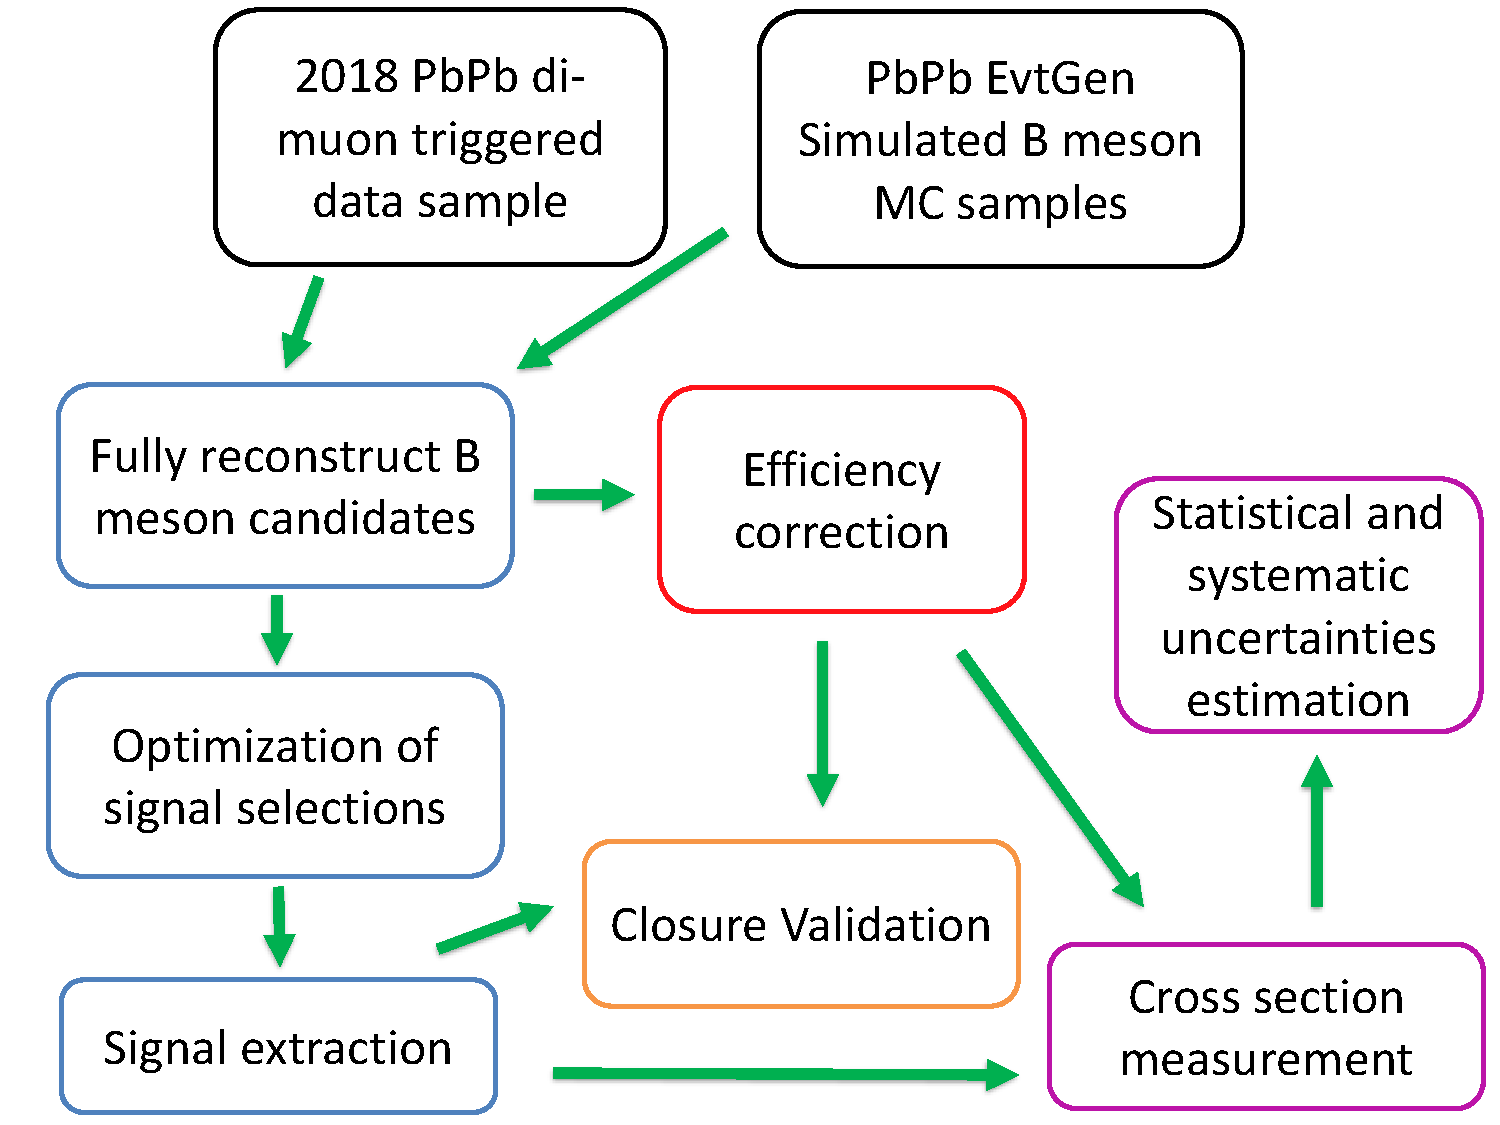
\includegraphics[width=0.65\textwidth]{Figures/Chapter4/BsBPWorkFlow.pdf}
\caption{The block diagram of the workflow with major steps for both B-meson cross section measurement is shown above.}
\label{BsBPWorkFlow}
\end{center}
\end{figure} 

Figure \ref{BsBPRECO} shows pictorially the decay topology of fully reconstructed B meson and our reconstruction strategies

\begin{figure}[hbtp]
\begin{center}
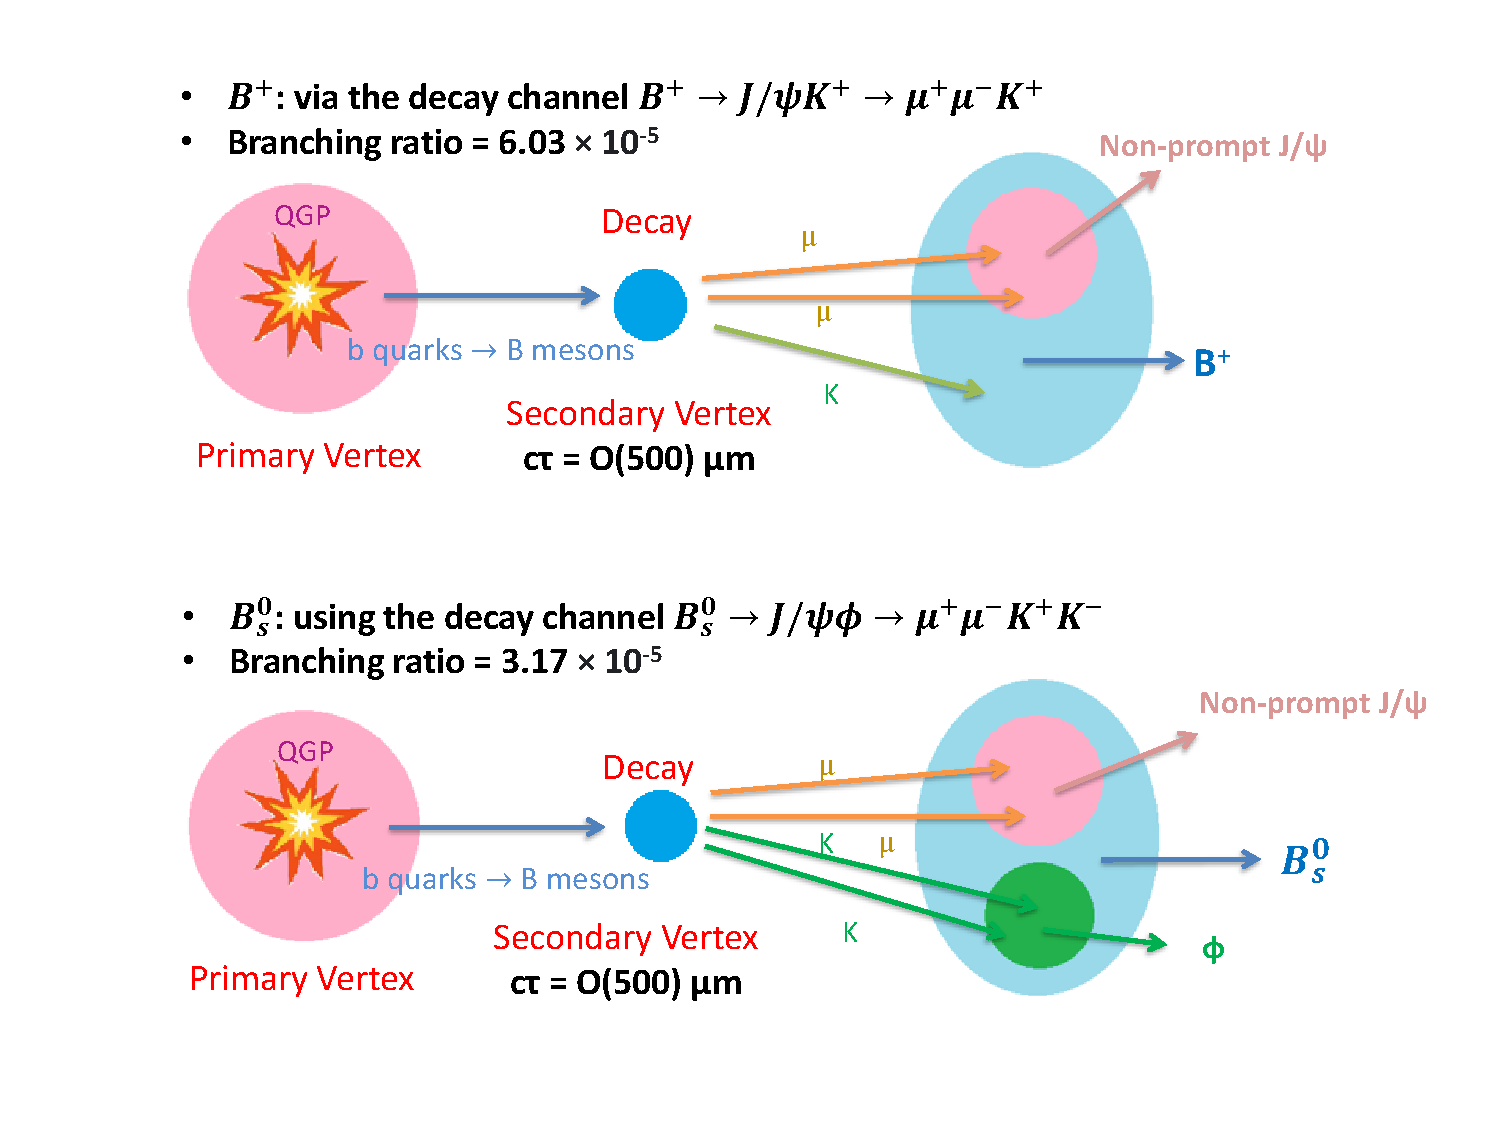
\includegraphics[width=0.86\textwidth]{Figures/Chapter4/BsBPRECO.pdf}
\caption{The strategies to fully reconstruct $B^0_s$ and $B^+$ in the selected exclusive decay modes are shown above.}
\label{BsBPRECO}
\end{center}
\end{figure} 


\subsection{Technical Challenges}

Despite the excellent muon, tracking, vertexing capabilities of the CMS detector, there are still many challenges for the analysis. Below is a list of challenges in the B-meson analysis 

\begin{itemize}
\item The small B meson decay branching ratio, which on in the order of 10$^{-5}$, and limited luminosity of the sample: $S \downarrow$ 
\item Huge combinatorial background without hadron particle identification, particularly in PbPb collisions and at low $p_T$:  $B \uparrow$ 
\item Low muon acceptance of at very low $p_T$: $S \downarrow$ 
\item High fake track rate with low tracking efficiency at very low $p_T$: $B \uparrow$ 
\end{itemize}

Here, $S$ stands for signal and $B$ stands for background. These factors will all lower the signal-to-background ratio, which makes challenging to fully reconstruct B mesons, particularly at very low $p_T$. In this thesis, to reduce the signal to background ratio and the systematic uncertainties, we will employ a novel approaching machine learning with multivariate analysis and the elaborated single particle efficiency correction method to perform the measurements.


\section{Analysis Samples}


\subsection{Dimuon Triggered Datasets}

In this part of the thesis, I focus on the studying beauty production and hadronization in QGP. Therefore, this analysis is performed using the 2018 PbPb data at $\sqrt{s_{NN}}$=5.02 TeV, which has an integrated luminosity of 1.7 $nb^{-1}$. 
The analysis uses the dimuon primary datasets (\textit{DoubleMu} PD). The full name of the used datasets and their corresponding luminosity can be found in Table~\ref{tab:lumi}.

\begin{table}[htb]
\begin{center}
\caption{List of PbPb HLT datasets and triggers with the corresponding integrated luminosities used in the analysis.}
\label{tab:lumi}
 \tiny
 \begin{tabular}{ l | l | l | l | }
 System& Primary dataset & Trigger & Luminosity\\
  \hline\hline 
PbPb & \verb#/HIDoubleMuonPsiPeri/HIRun2018A-04Apr2019-v1/AOD# & \verb# HLT_HIL3Mu0NHitQ10_L2Mu0_MAXdR3p5_M1to5_v1 # & 522 $nb^{-1}$\\
  PbPb & \verb#/HIDoubleMuon/HIRun2018A-04Apr2019-v1/AOD # & \verb# HLT_HIL3Mu0NHitQ10_L2Mu0_MAXdR3p5_M1to5_v1 # & 1124 $nb^{-1}$ \\
  \hline
  PbPb & Combined All & & 1.657 ($\sim$ 1.7) $nb^{-1}$ \\
 \end{tabular}
\end{center}
\end{table}

The details of the dimuon trigger selection to collect the data sample is explained in 2.2.5. In addition, an Muon JSON to select good luminosity sections in the PbPb dataset is applied. Both $B^0_s$ and $B^+$ data come from this sample. However, in the later stage, the B meson candidates are saved in different channels based on the reconstruction.

\subsection{Monte Carlo Simulations Samples}

Dedicated PbPb $B^0_s$ and $B^+$ samples are generated in order to estimate the acceptance and selection efficiencies, to study the background components, and to evaluate systematic uncertainties. {\sc PYTHIA8} Tune CUETPM8~\cite{PYTHIAFrag,PYTHIA2}, set to generate inclusive (all quark/antiquark, as well as gluon initiated) QCD processes, was used to generate at 5.02 TeV the signal. Several preselections at the generation steps are applied in order to optimize the generation process and conserve resources.

For $B^0_s$, only signal events were kept with at least one $B^0_s$ (forced to decay through the channel $B^0_s \rightarrow J/\psi \phi \rightarrow \mu^+\mu^-K^+K^-$ by means of the {\sc evtgen} package~\cite{EvtGen}), with $p_{T}>$ 5.0 GeV/c, and $|\eta|<$ 2.4. In addition, the $J/\psi$ and $\phi$ meson, are forced to decay in the two muons and two kaons respectively. Final state radiations are generated using {\sc photos}~\cite{PHOTOS}. The selected signal B mesons {\sc PYTHIA8} events were embedded into a PbPb background simulated with the {\sc HYDJET}  (version 1.8, tune ``Drum'' for the prompt and non-prompt $J/\psi$ MC and tune "Cymbal5Ev8" for the $B^0_s$ signal MC)~\cite{HYDJET} event generator.

For $B^+$, similar requirements for MC generation are applied except a different decay channel $B^0_s \rightarrow J/\psi K^+ \rightarrow \mu^+\mu^-K^+$ is used.

For $B^0_s$ and $B^+$, around fifty thousand events were generated in 5 $\hat{p}_{T}$ bins, with boundaries of $\hat{p}_{T} >$ 0, 5, 15, 30, 50, in both signal only, and embedded samples. The high $\hat{p}_{T}$ selections are used to enrich the high $p_T$ B meson statistics in order to perform efficiency correction. 

We should note that in there are two components in the MC sample. The truth information about the particles generated in the simulation, which is call generated (GEN), and the reconstructed one smeared according to the CMS detector effects, which is called reconstructed (RECO). Due to the nature of MC generation, we will need to reweigh on MC in order to model the data.

In addition to the $B^0_s$ and $B^+$, a sample of inclusive b hadron to $J/\psi$ (non-prompt) MC is also simulated to study the possible background contribution to the B-meson analysis due to 


\subsection{$\hat{p}_{T}$ Reweighing}


As we mention above, different $\hat{p}_{T}$ cut is applied to generate the MC samples. When merging the samplings, a  $\hat{p}_{T}$ weight based on beauty production cross section is required to apply to the MC in order to obtain a smooth distribution that can model the real data. Figure \ref{GENPTDIS} shows the generated $p_T$ ($Gp_T$) distribution of $J/\psi$, $B^+$ , and $B^0_s$ before and after applying the $\hat{p}_{T}$ weight:


\begin{figure}[h]
\begin{center}
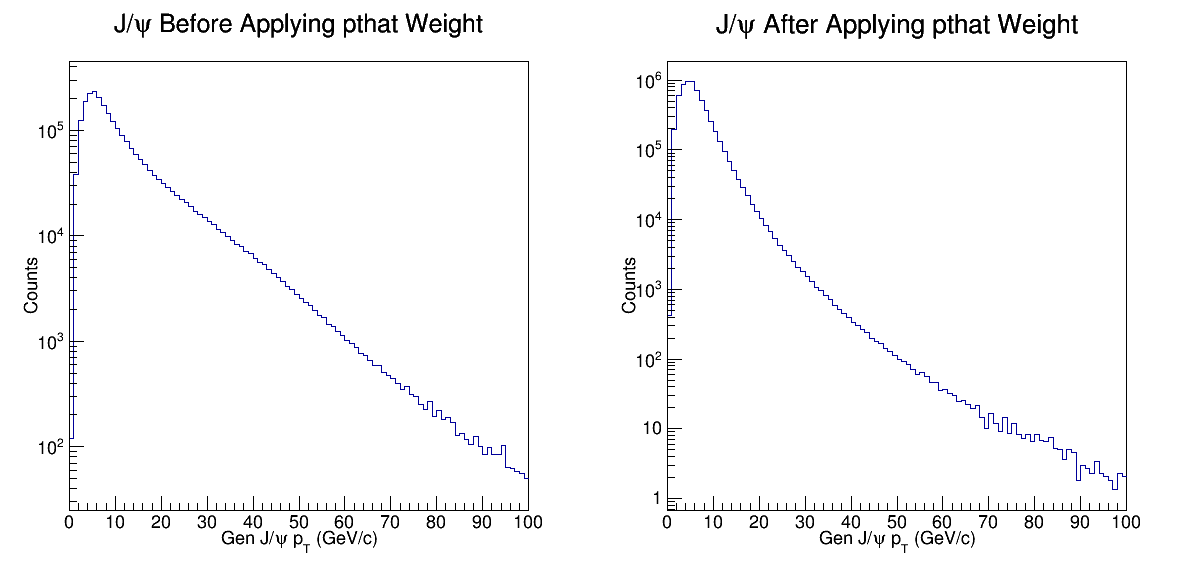
\includegraphics[width= 0.90\textwidth]{Figures/Chapter4/JPsiGenpT.png}
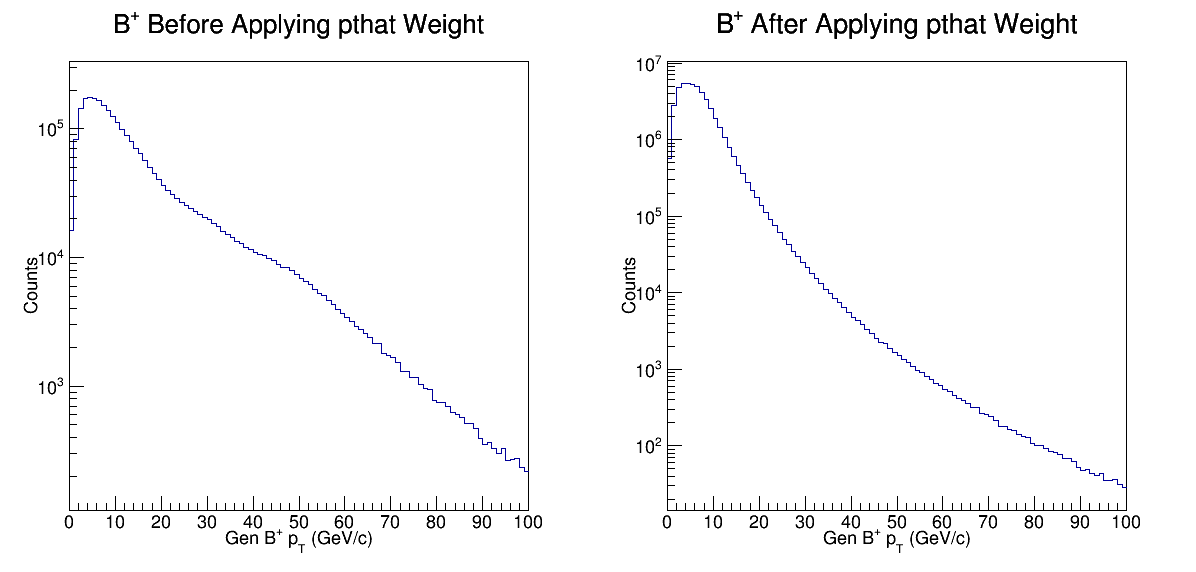
\includegraphics[width= 0.90\textwidth]{Figures/Chapter4/BPlusGenpT.png}
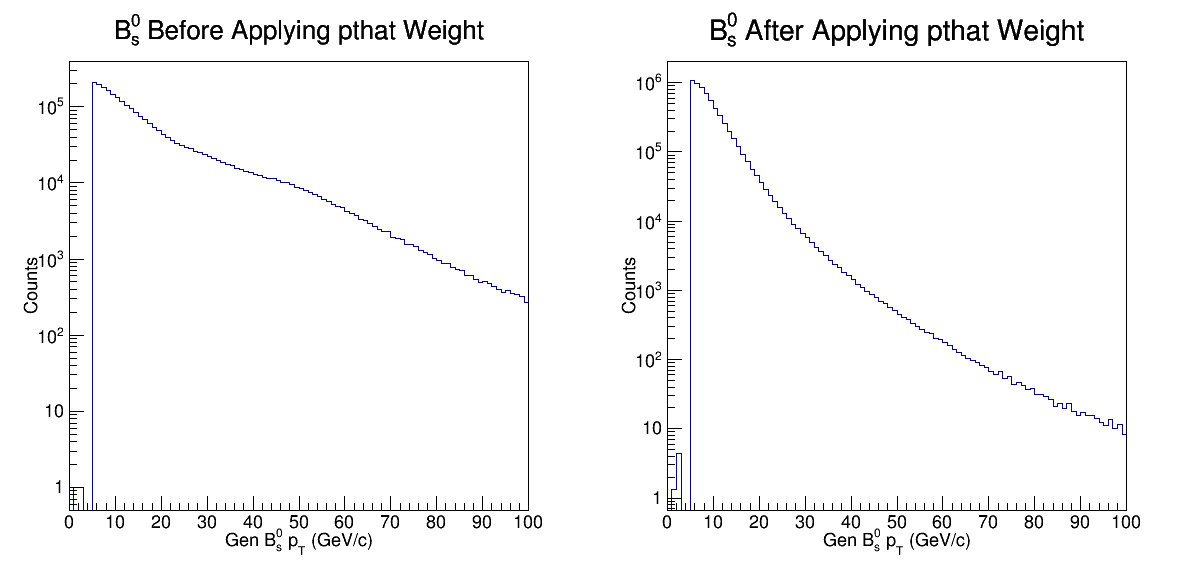
\includegraphics[width= 0.90\textwidth]{Figures/Chapter4/BsGenpT.png}
\caption{ $J/\psi$ generated $p_{T}$ distribution before (upper left) and after (upper right) $\hat p_{T}$ reweighing, $B^+$ generated $p_{T}$ distribution before (middle left) and after (middle right) $\hat p_{T}$ reweighing, and $B_s^0$ generated $Gp_{T}$ distribution before (lower left) and after (lower right) $\hat p_{T}$ reweighing are shown above.}
\label{GENPTDIS}
\end{center}
\end{figure}


\subsection{RECO B-meson ${p}_{T}$ Reweighing}

Then, we also check if this smooth $Gp_T$ shape in fact correspond to a good agreement between the data and MC in the RECO side. Therefore, we take the ratio of the normalized data raw yield to the normalized MC raw yield and perform a variety of functions to fit the distribution. In our studies, we use Linear ($y = p_0 + p_1 x$), Quadratic ($y = p_0 + p_1 x + p_2 x^2$), Linear + Inverse  ($y = p_1 x + \frac{p_2}{x}$), Linear + Square Root ($y = p_0 + p_1 x + p_2 \sqrt{x}$), Linear + Log ($y = p_0 + p_1 x + p_2 \log{x}$). The data vs MC raw yield shape and our fitting results on spectra ratio are show as follows \ref{BsBptWeight} and  \ref{BPBptWeight} for $B^0_s$ and $B^+$ respectfully 



\begin{figure}[h]
\begin{center}
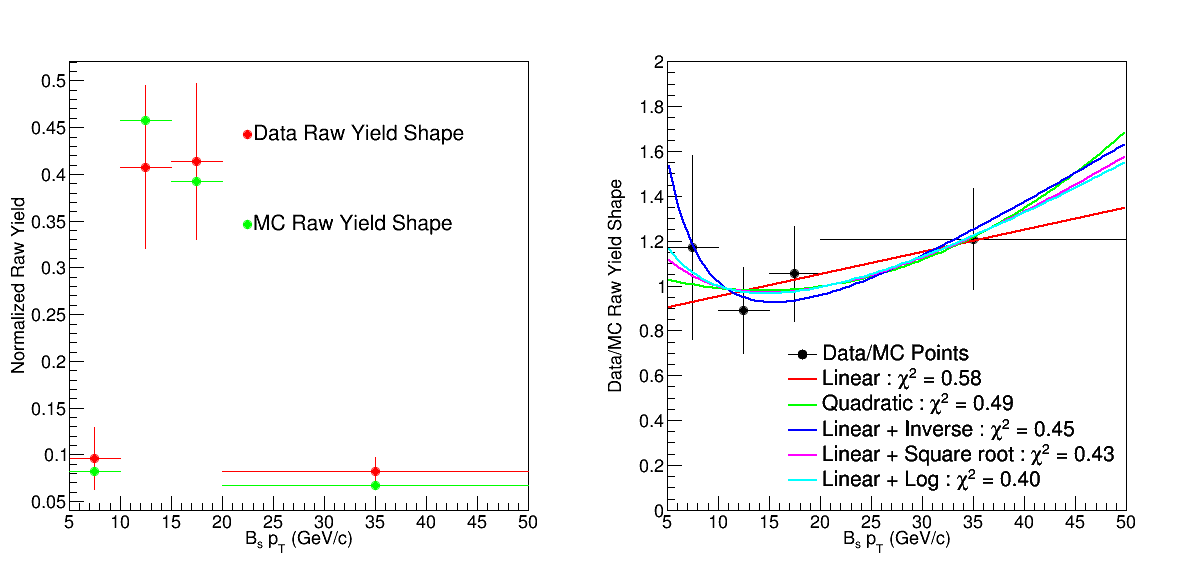
\includegraphics[width= 0.97\textwidth]{Figures/Chapter4/BsBptDataMC.png}
%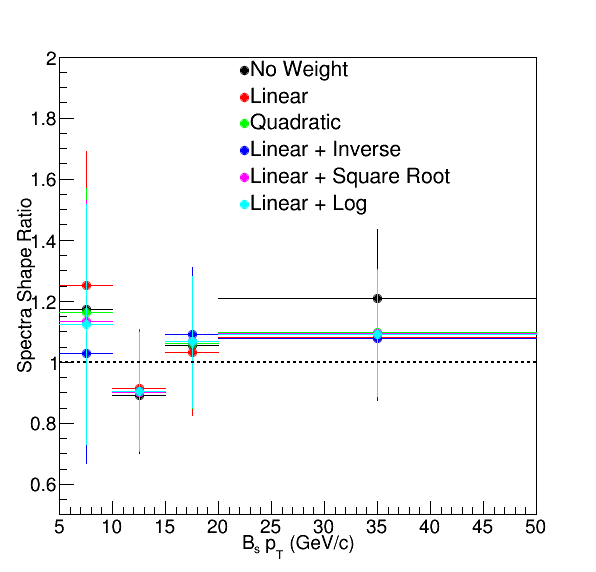
\includegraphics[width= 0.55\textwidth]{Figures/Chapter4/BsBptDataMCAfter.png}
%\caption{ $B^0_s$ $p_T$ normalized raw yields obtained in PbPb MC and Data are shown above on the top left panel. The data/MC ratio and different fitting functions: Linear (Red), Quadratic(Green), Linear + Inverse (Blue), Linear + Square Root (Purple), and Linear + Log (Cyan) and their $\chi^2$ are shown above on the top right panel. The bottom plots are the data/MC reweighed yields with different functions from the fit on the top right panel. We can see that they all get closer to unity compared unweighted MC. The Linear + Log (Cyan) line, which has the smallest $\chi^2$ and is closest to unity after applying the weight to the MC. Hence, Linear + Log function is use as nominal for our $B^0_s$ $p_{T}$ reweighing. All other fitting function are used as reference to calculate the $p_T$ shape systematic uncertainties.}
\caption{ $B^0_s$ $p_T$ normalized raw yields obtained in PbPb MC and Data are shown above on the top left panel. The data/MC ratio and different fitting functions: Linear (Red), Quadratic(Green), Linear + Inverse (Blue), Linear + Square Root (Purple), and Linear + Log (Cyan) and their $\chi^2$ are shown above on the top right panel. The bottom plots are the data/MC reweighed yields with different functions from the fit on the top right panel.}
\label{BsBptWeight}
\end{center}
\end{figure}

\begin{figure}[h]
\begin{center}
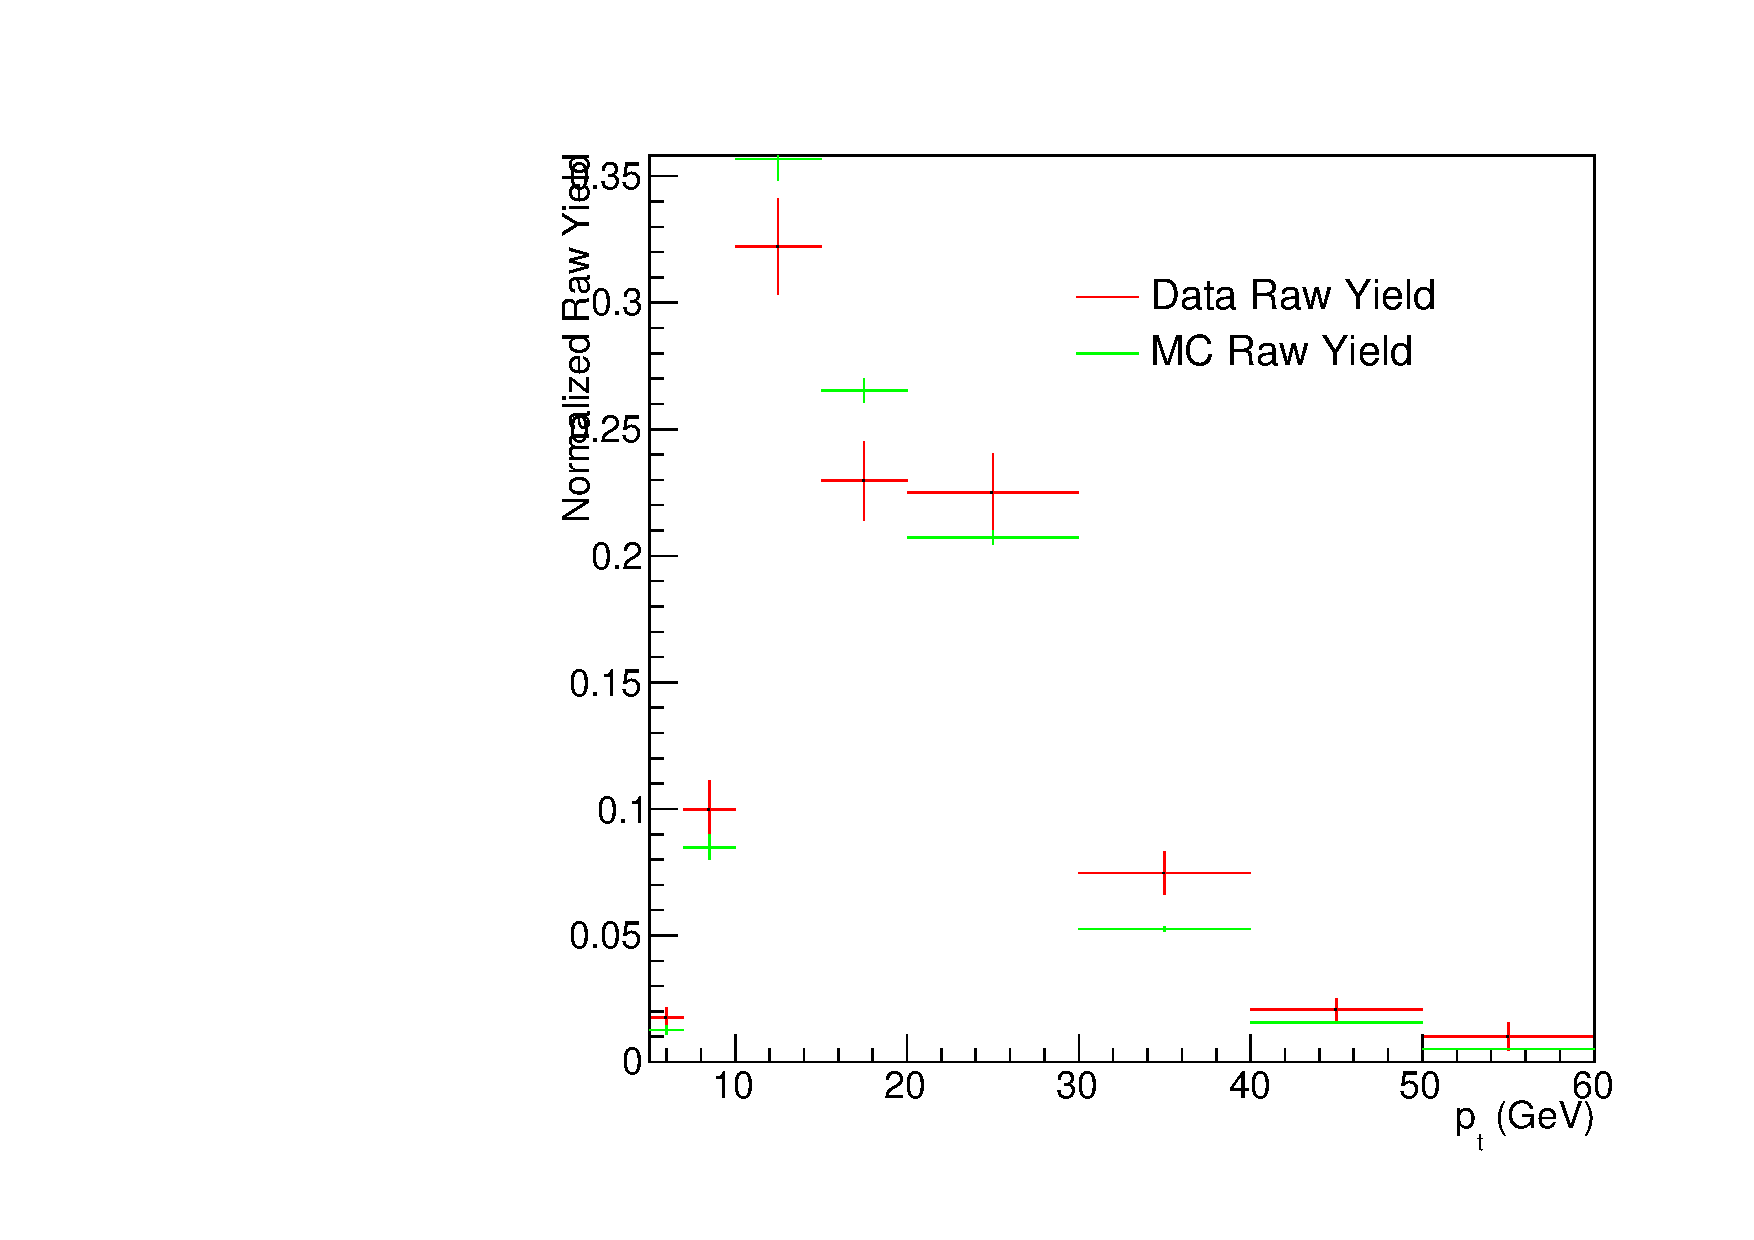
\includegraphics[width= 0.48\textwidth]{Figures/Chapter4/BPBptDataMC1.pdf}
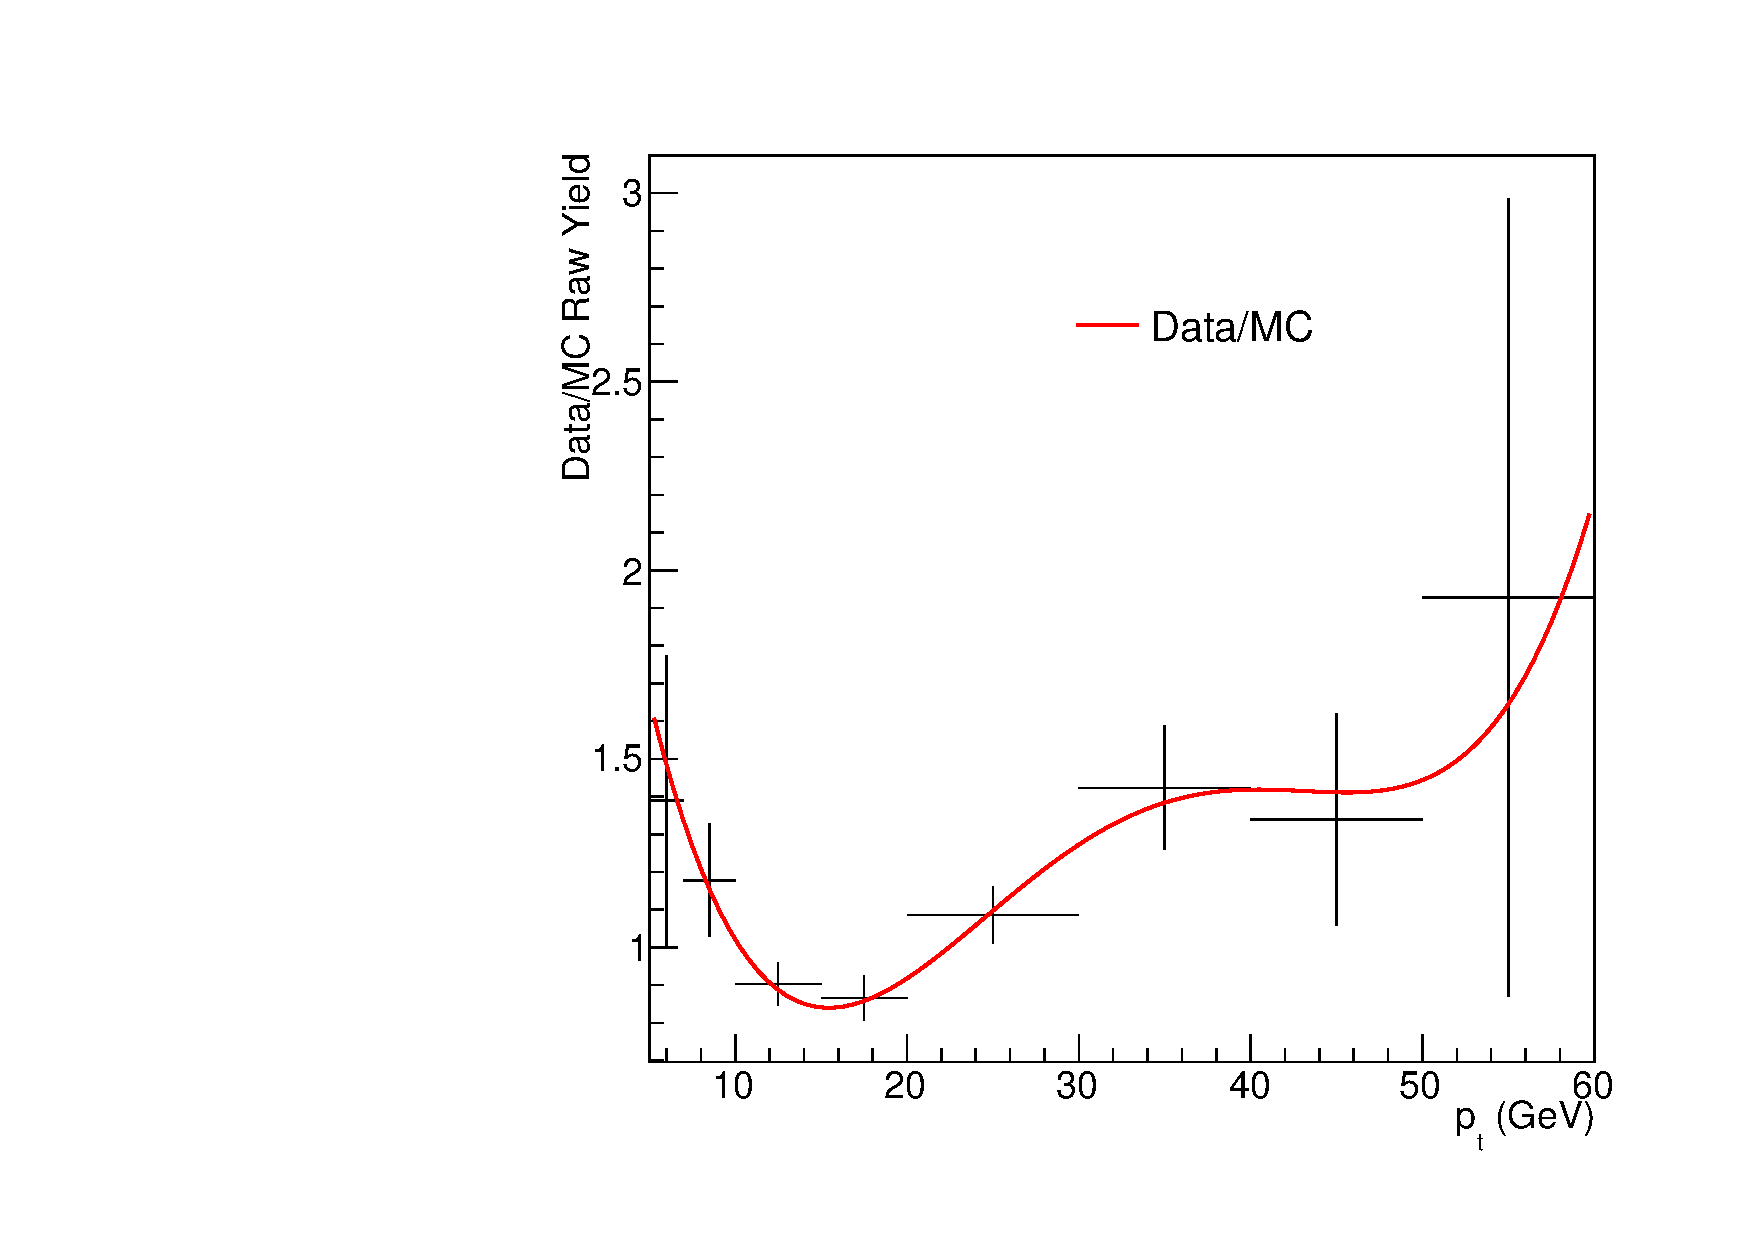
\includegraphics[width= 0.48\textwidth]{Figures/Chapter4/BPBptDataMC2.pdf}
\caption{The normalized $B^+$ raw yield in MC (green) and Data (red) as a function RECO $B^+$ $p_T$ (left) and the fourth order polynomial fits to their ratio (right) are shown above.}
\label{BPBptWeight}
\end{center}
\end{figure}


\subsection{Centrality Reweighing}

Because the MC simulations employ PYTHIA embedded into a PbPb background simulated, they do not model the centrality of nucleus-nucleus collision well. Therefore, the MC simulations are also reweighed in order to match the centrality distribution in data. In the middle panel of Figure \ref{CentComp}, the centrality distribution of the MC simulation (red) is compared to the one in data (blue), before the re-weighting. Each unit (hiBin) on the x-axis represents 0.5\% centrality. The number of binary collisions $N_{coll}$ was used as the weight to scale the MC centrality, and the distribution presented in the right panel of Figure 4 was obtained. 

\begin{figure}[hbtp]
\begin{center}
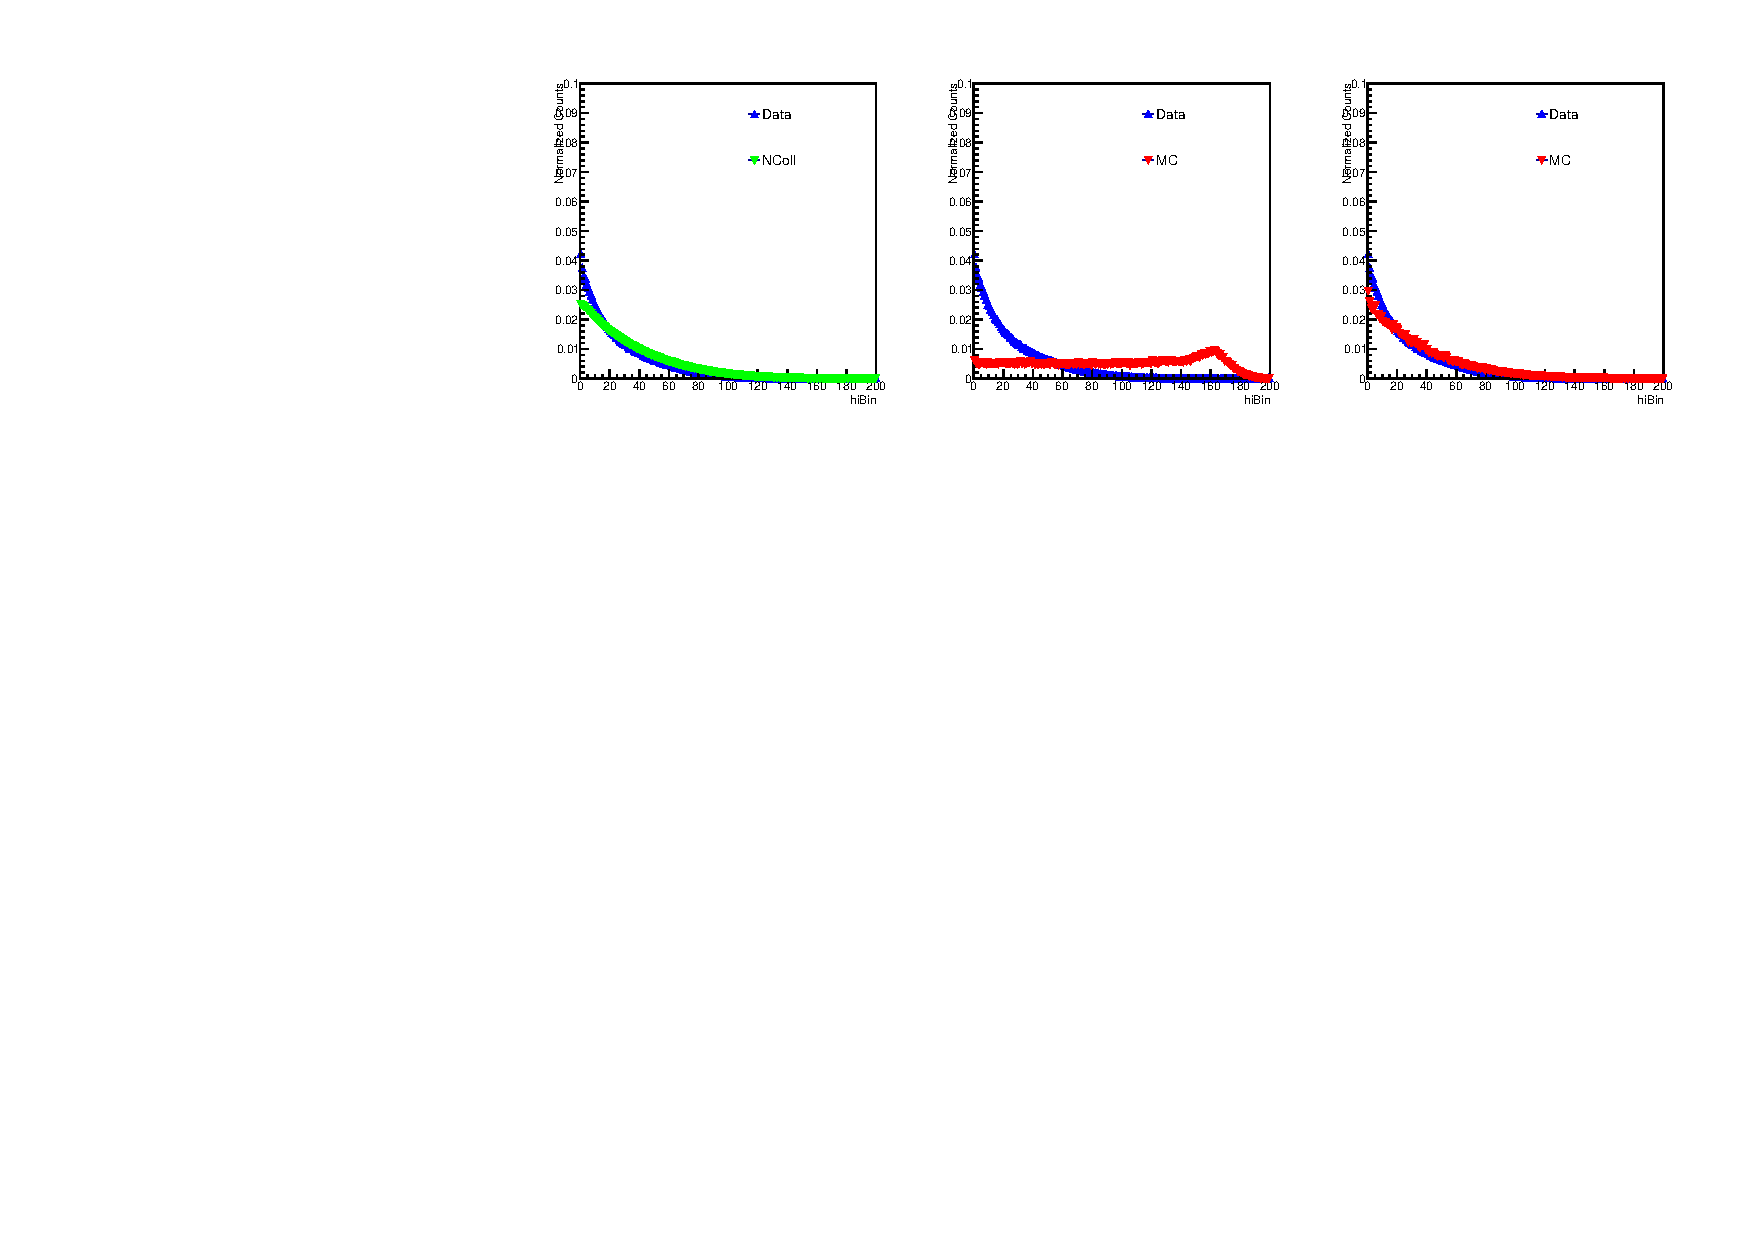
\includegraphics[width=1.10\textwidth]{Figures/Chapter4/CentralityWeight.pdf}
\caption{The comparison between $N_{coll}$ and Data vs hiBin (left), centrality distribution of MC (red) and data (blue) in PbPb collisions in the centrality interval 0-100\% without $N_{coll}$ weight (middle), and with $N_{coll}$ weight (right) are shown above.}
\label{CentComp}
\end{center}
\end{figure} 


A better centrality agreement between the data and the MC is seen after the reweighing process. 

\subsection{PV$_{z}$ Reweighing}


In addition to above pt shape and centrality reweighing, there must be a primary vertex $z$ position (PV$_{z}$) reweighing due to incorrect modeling of the primary vertex location and resolution in the MC simulation. In fact, it is known that the MB samples use for embedding for PbPb signal MC samples (with Cymbal5Ev8 tune) has a PV$_{z}$ offset. Also, the offsets between data and MC in the X and Y directions are observed in the 2018 PbPb collisions. To remedy this, a Gaussian fit is applied to both the data and MC PV$_{z}$ distributions, as showed in Fig.~\ref{PVZPlot}. The black markers represent the distribution points for MC (left), and data (right), while the red line represents the fit result. Then, the ratio between the two fit results is taken as the weighting function. The result after this weighting can be found in Fig. \ref{PVZPlot} But we should note that this analysis is not sensitive to the absolute value of the PV position because the reconstruction of the B-meson rely only on the relative distance between PV and B-meson reconstructed vertex which will be presented in the later sections.

\begin{figure}
\begin{center}
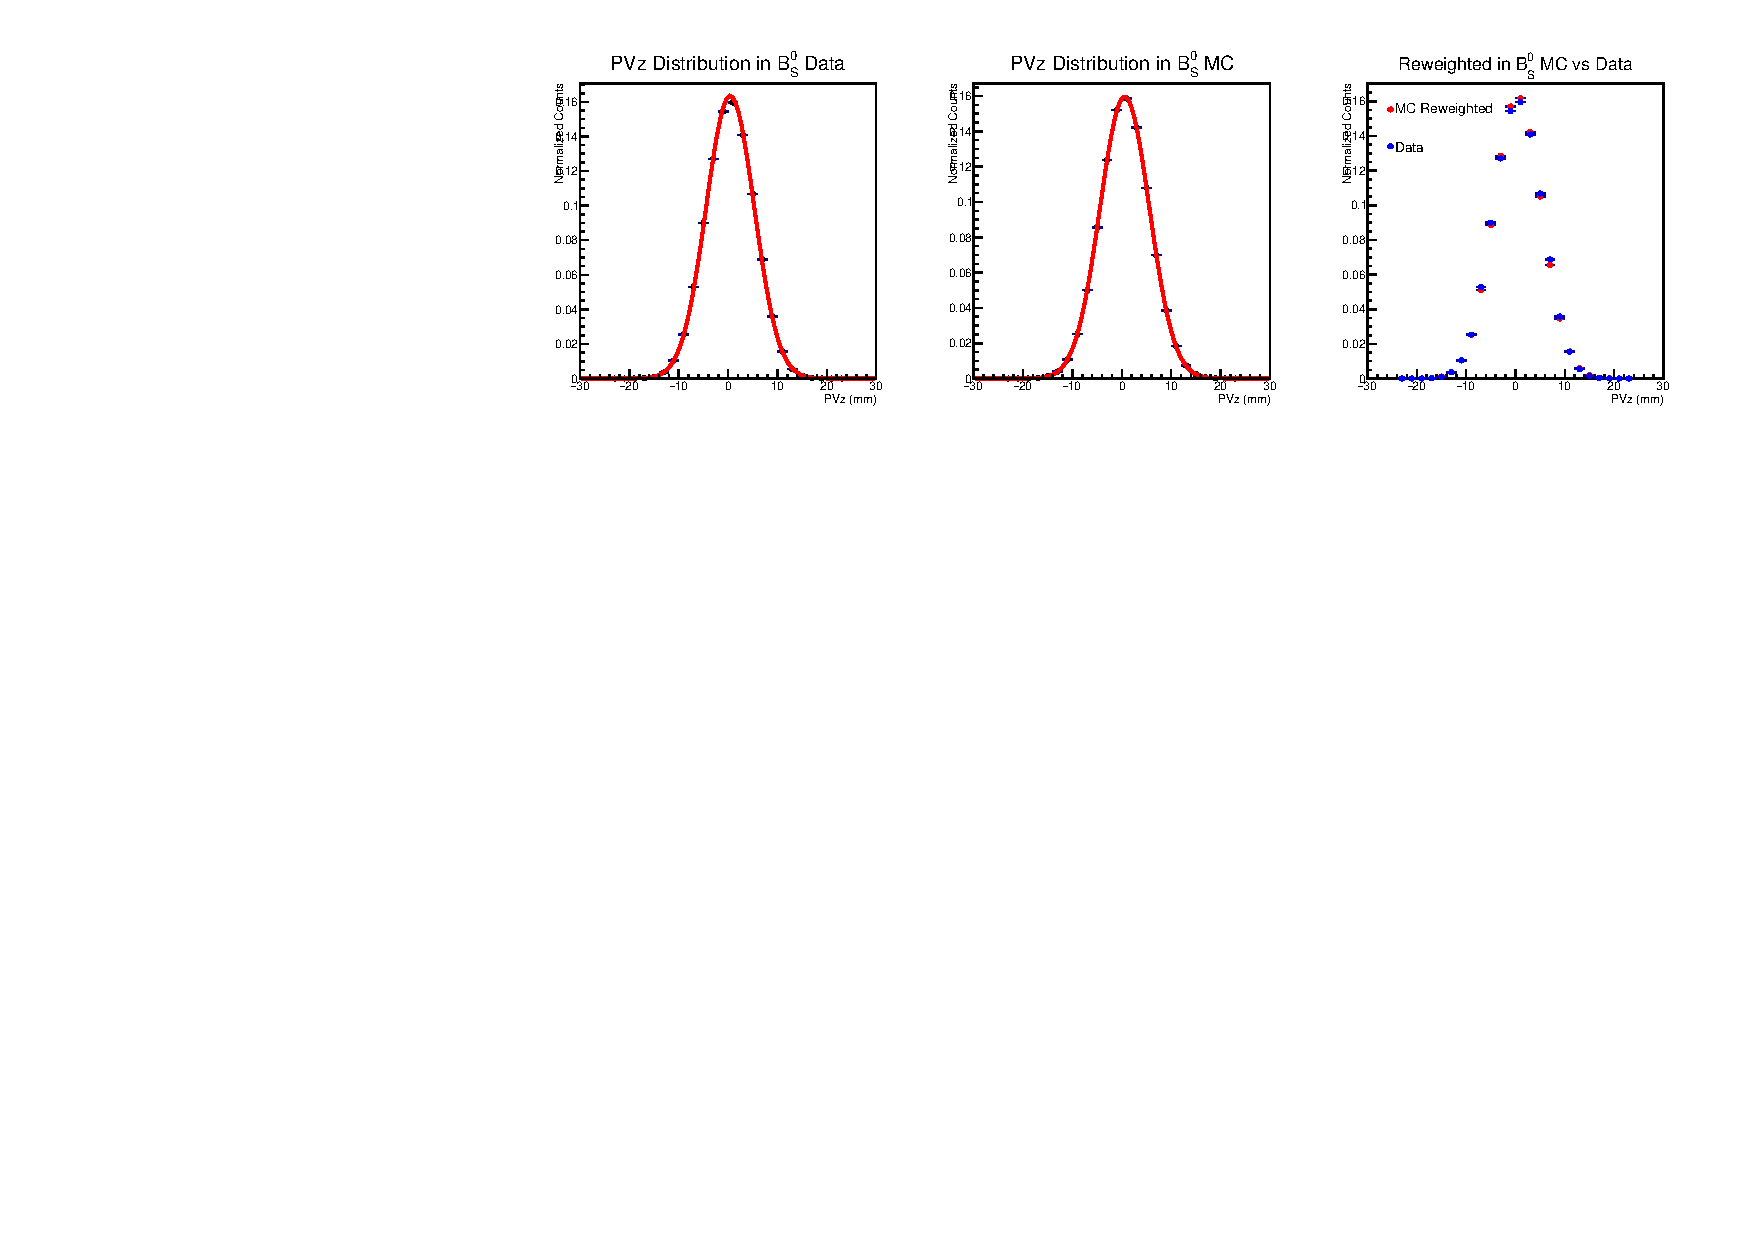
\includegraphics[width= 1.10\textwidth]{Figures/Chapter4/PVzWeightPbPb.pdf}
\caption{Primary vertex z position (PV$_{z}$) distribution, fitted with a gaussian function in PbPb MC simulations (left), in PbPb data (middle), PV$_{z}$ reweighed MC to data with ratio of data-to-MC Gaussian Fits (right) are shown above. The PV$_z$ distributions are well described by the Gaussian function and reweighing reduces the MC-data discrepancy.}
\label{PVZPlot}
\end{center}
\end{figure}

A almost perfect MC-data agreement after PV$_{z}$ reweighed is observed above. After these standard reweighing procedures, the residue disagreement between MC and data will be considered as a source of systematic uncertainties.


\clearpage

\section{Global Event Observables} 

The global event observables characterize general conditions of heavy-ion collision. In this analysis, we decide to use another set of quantities including total number of MB events to represent the luminosity and average number of participants $N_{parts}$ to represent centrality. In addition, to compare with $pp$ collisions, we also need to scale the cross section in PbPb according to . Therefore, we will determine the all the global event observable including total number of minimum bias events ($N_{MB}$), centrality, number of participant nucleons $N_{part}$, number of binary collisions $N_{coll}$, and nuclear overlapping function $T_{AA}$ in dimuon PbPb dataset in the follow subsections.

\subsection{Total Number of Events}

As seen in Table \ref{tab:lumi}, the nominal luminosity of the dimuon PbPb dataset 1.7 $nb^{-1}$. However, this nominal luminosity has large uncertainties and should be used in the analysis to measure the cross section. As mentioned previous in Chapter 2.2, the dimuon trigger, based on the MB trigger, will not save events that does not pass trigger selections. Hence, we can use the events of 1 PD MB datasets (PD0) via the follow formula to determine the actual number of MB events corresponding to the dimuon PbPb datasets: 


\begin{equation}
N_{MB} = \frac{N^{\mu\mu json}_{MB}}{\mathcal{L}_{MB trigger}^{\mu json}} \mathcal{L}_{\mu\mu trigger}^{\mu\mu json}
\end{equation}

The definition of the variables in the formula are as follows:


\textbf{$N_{MB}$:} The number of minimum bias events in dimuon PD with muon json.

\textbf{$N^{\mu json}_{MB}$:} The number of event of all MB PDs with muon json. 

\textbf{$\mathcal{L}^{\mu json}_{MB}$:} The luminosity of all MB PDs with muon json.

\textbf{$\mathcal{L}_{\mu\mu trigger}^{\mu\mu json}$:} The luminosity of dimuon PD with muon json.

\iffalse 

To obtain the total number of minimum bias $N_{MB}$, first we process one PD (PD5) minimum bias events and count the total number of events for centrality at 0 - 90\% to obtain $N^{\mu\mu json}_{MB}$. Then, we run the brilcal for MB PD5 and sum the luminosity of HLT MB triggers: 

Trigger 1: ``HLT\_HIMinimumBias\_part0\_v1" 
 
Trigger 2: ``HLT\_HIMinimumBias\_SinglePixelTrack\_part0\_v1"
 
Trigger 3: ``HLT\_HIMinimumBias\_SinglePixelTrack\_NpixBypass\_part0\_v1" 
  
Trigger 4: ``HLT\_HIMinimumBias\_SinglePixelTrack\_NpixGated\_part0\_v1" 
 
to obtain $\mathcal{L}^{\mu\mu json}_{MB}$. 

Trigger 5: ``HLT\_HIL3Mu0NHitQ10\_L2Mu0\_MAXdR3p5\_M1to5\_v1" 

to obtain $\mathcal{L}^{\mu\mu json}_{MB}$. 

Table ~\ref{tab:lumibreadown} shows the luminosity of Trigger 1 -- 5 above. The sum of trigger 1 -- 4 will be $\mathcal{L}^{\mu\mu json}_{MB}$ and trigger 5 will be $\mathcal{L}^{\mu\mu json}_{MB}$.

\begin{table}[h]
\begin{center}
\caption{Summary table of the luminosity of HLT triggers to obtain the number of minimum biased events.}
\vspace{1em}
\label{tab:lumibreadown}
  \begin{tabular}{ |c | c| }
      \hline
   HLT  & Luminosity ($\mu b^{-1}$)  \\
    \hline
    \hline 
 HLT\_HIMinimumBias\_part0\_v1        & 14.8269  \\
 `HLT\_HIMinimumBias\_SinglePixelTrack\_part0\_v1  & 1.3010  \\
HLT\_HIMinimumBias\_SinglePixelTrack\_NpixBypass\_part0\_v1 & 7.9468 \\
HLT\_HIMinimumBias\_SinglePixelTrack\_NpixGated\_part0\_v1 &  \\
    \hline 
Total & 24.0748  \\
    \hline 
HLT\_HIL3Mu0NHitQ10\_L2Mu0\_MAXdR3p5\_M1to5\_v1  & 1657.1320 \\
     \hline
    \hline
\end{tabular}
\end{center}
\end{table}


We have also obtained the number of events by processing one of the MB sample. The total number of events can be found in Table \ref{tab:NMBEventsCent}. 

\begin{table}[h]
\begin{center}
\caption{Summary table of the total number of MB events vs centrality}
\vspace{1em}
\label{tab:NMBEventsCent}
  \begin{tabular}{ |c | c| }
    \hline 
Centrality & $ \mathcal{L}_{\mu\mu trigger}^{\mu\mu json}$ \\
     \hline
         \hline
0-10\% & 18276069  \\
10-20\%& 17680482  \\
20-30\% & 17687566 \\
30-40\% & 17684913 \\
40-50\% & 17685909 \\
50-60\% & 17680807 \\
60-70\% & 17686640 \\
70-80\% & 18375623 \\
80-90\% & 18749965 \\
0-30\% & 53644117 \\
30-90\% & 107863857 \\
0-90\% & 161507974 \\
     \hline
    \hline
\end{tabular}
\end{center}
\end{table}

\fi

For 0 - 90\%, $N_{MB}^{\mu json}$ is 161507974. The number of events can then be computed as follows:

\begin{equation}
N_{MB} = \frac{N^{\mu json}_{MB}}{\mathcal{L}_{MB trigger}^{\mu json}} \mathcal{L}_{\mu\mu trigger}^{\mu json} = \frac{1657.1320 \mu b^{-1}}{24.0748  \mu b^{-1}} \times 161507974 =  1.1823737719 \times 10^{10} \simeq  \textbf{11.82 billion}
\end{equation}

Hence, the number of MB event for the dimuon PbPb data is $N_{MB} = $11.82 billion. Below, in Table \ref{NMBUsedCent}, we compile the number of minimum biased events $N_{MB}$ in 0 - 30\%, 30\% - 90\%,and 0 -90\%. 

\begin{table}[h]
\begin{center}
\caption{Summary table of the total number of MB events vs centrality}
\vspace{1em}
\label{NMBUsedCent}
  \begin{tabular}{ |c | c| }
    \hline 
Centrality & $N_{MB}$ (billion) \\
     \hline
         \hline
0-30\% &  3.941 \\
30-90\% & 7.882 \\
0-90\% & 11.82 \\
     \hline
    \hline
\end{tabular}
\end{center}
\end{table}

%According to the official results from the CMS Global Observable Group, the number of events we obtains is about $N_{events} =$ 11968044281 $\simeq$ 12.0 billion for (0 - 90\%) centrality from using the brilcal to evaluate the luminosity and process MB PD0--5 with our muon JSON, which is very close our calculations: $N_{events} =$ 11.82 billion. Here, we will use the official results

\subsection{Centrality Definition}

For the 2018 PbPb dataset, the centrality is given in hiBin with 0.5\% increment. The hiBin is defined based on the HF response (hiHF). According to the Global observable, \ref{hiHFvsCent} is the hiHF as a function of centrality with uncertainties.


\begin{figure}[h]
\begin{center}
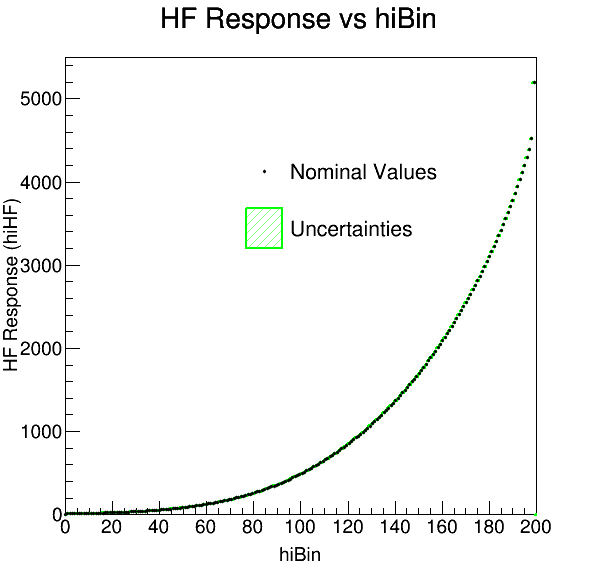
\includegraphics[width= 0.48\textwidth]{Figures/Chapter4/hiHFvsCent.png}
\caption{The nominal (black) and uncertainties band (green) hiHF vs hiBin for CMS 2018 PbPb dataset are shown above.}
\label{hiHFvsCent}
\end{center}
\end{figure}


We can compute the percent deviation nom of final results to estimate systematics due to uncertainties of centrality. 


\subsection{$\langle N_{part} \rangle$, $\langle N_{coll} \rangle$, $\langle T_{AA} \rangle$ vs Centrality}

As we discussed in the Glauber Model \cite{CentPlot,Glauber} section 1.5.7, the number of participant nucleons $N_{part}$, the number of binary nucleon-nucleon collisions, and nuclear over lapping function $T_{AA}$ are all functions of the event centrality. The CMS Global Observable group has computed the average $N_{part} $, $N_{coll} $, $T_{AA}$ and their uncertainties  for different centrality bins based on the Glauber Model. The selected results are shown Table \ref{GOvsCent} below


\begin{table}[h]
\begin{center}
\caption{Summary table of the total number of MB events vs centrality is shown below. The uncertainties are represented in terms of percentage in the parenthesis.}
\vspace{1em}
\label{GOvsCent}
  \begin{tabular}{ |c | c| c| c|}
    \hline 
Centrality &  $\langle N_{part} \rangle$ &$\langle N_{coll} \rangle$  & $\langle T_{AA} \rangle$  \\
     \hline
         \hline
0-30\% &  269.1 (0.39\%)  &  1042 (2.0\%) &	15.42 (2.0\%)   \\
30-90\% & 54.45 (1.5\%)   & 115.2 (3.6\%)  &   1.704 (3.6\%)  \\
0-90\% & 126.0 (0.67\%)   &  424.1(2.2\%)  &    6.274 (2.2\%)  \\
     \hline
    \hline
\end{tabular}
\end{center}
\end{table}

The global observables $N_{MB}$, $N_{part}$, $N_{coll}$, and $T_{AA}$ will be used inputs for our B-meson analysis. 

\iffalse

\subsection{Number of Participant Nucleons}

\subsection{Number of Binary Collisions}


\fi

\subsection{Event Multiplicity}

Aside from $N_{MB}$, $N_{part}$, $N_{coll}$, and $T_{AA}$, event multiplicity is also an event observable. We count the number of tracks in each event with some track quality selections and use it to interpret the event multiplicity, which characterizes the event activity. The following is the selection criteria for 

Nevertheless, the event multiplicity is not used in PbPb analysis. It will be used in $pp$ analysis to study the $B^0_s/B^+$ ratio as a function of event multiplicity in $pp$ collisions.

%\section{Monte Carlo Simulations} 

%The Monte Carlo (MC) simulation on the B meson decay is essential to the analysis. It will plays an important role in both the signal extraction and efficiency correction.

%\subsection{PYTHIA}

%\subsection{Hydjet Embedding}

%\subsection{EvtGen Package}

%\subsection{MC reweighing}

\section{B meson Reconstruction} 

Now we look into each events of the PbPb dimuon dataset. It turns out that there is no PU in any event. Therefore, only one primary vertex for each event. We can then reconstruct the B meson candidates according to the final state muons and kaons tracks. In CMS, a dedicated software named ``\textit{Bfinder}'' is developed to perform B-meson reconstruction. Figure \ref{BsRECOWF} and \ref{BPRECOWF} show the workflow to fully reconstruct \textit{Bfinder} for $B^0_s$ and $B^+$ respectfully.


\begin{figure}[h]
\begin{center}
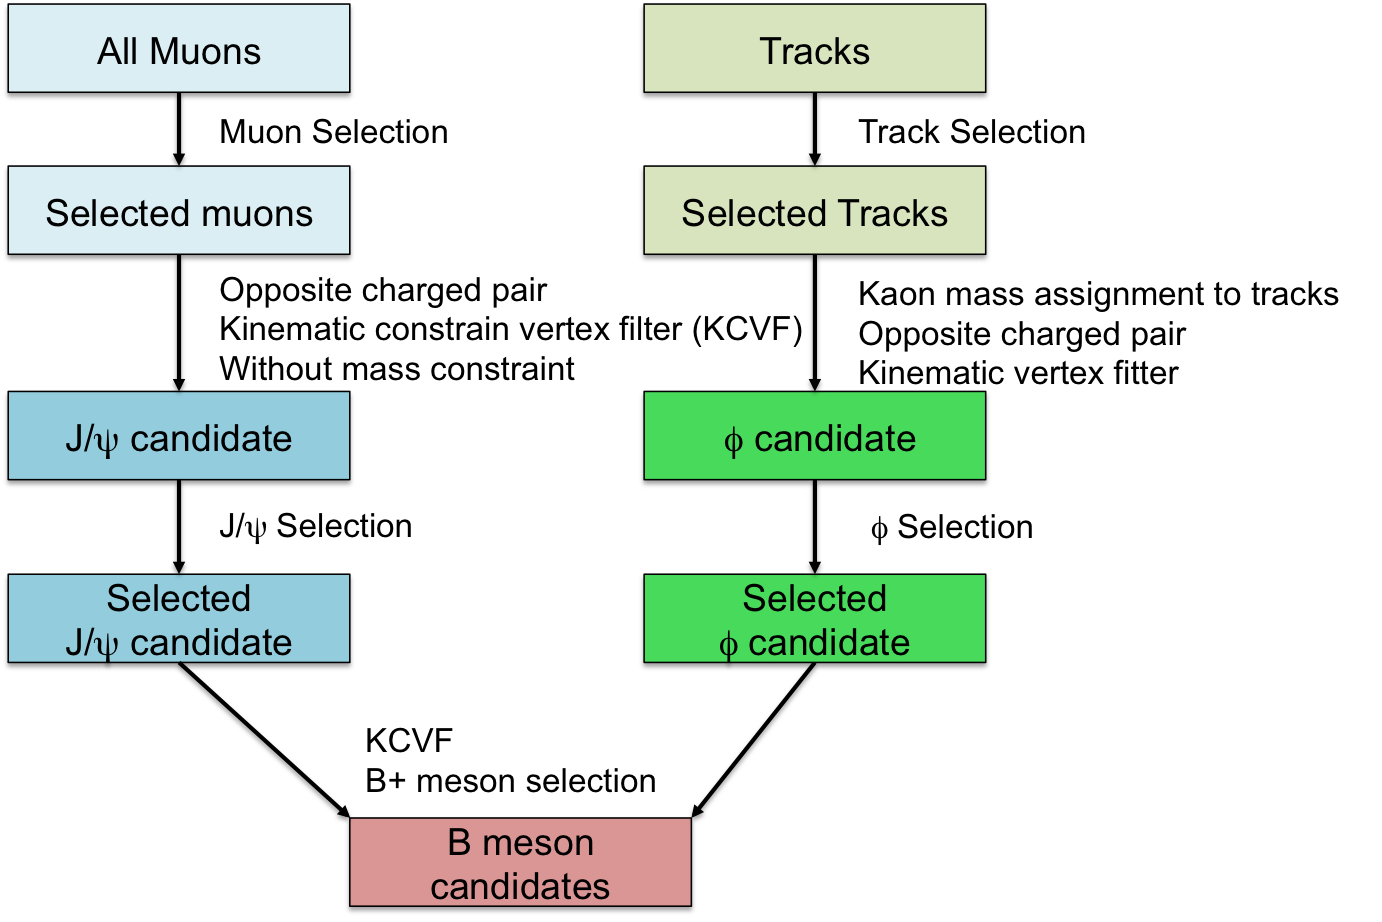
\includegraphics[width= 0.98\textwidth]{Figures/Chapter4/BsmesonWorkflow.png}
\caption{The schematic block diagram of the full reconstruction workflows for $B^0_s$ via the decay channel of $B_s^0 \rightarrow J/\psi \phi \rightarrow \mu^+\mu^- K^+K^-$ in the \textit{Bfinder} is shown above.}
\label{BsRECOWF}
\end{center}
\end{figure}

\begin{figure}[h]
\begin{center}
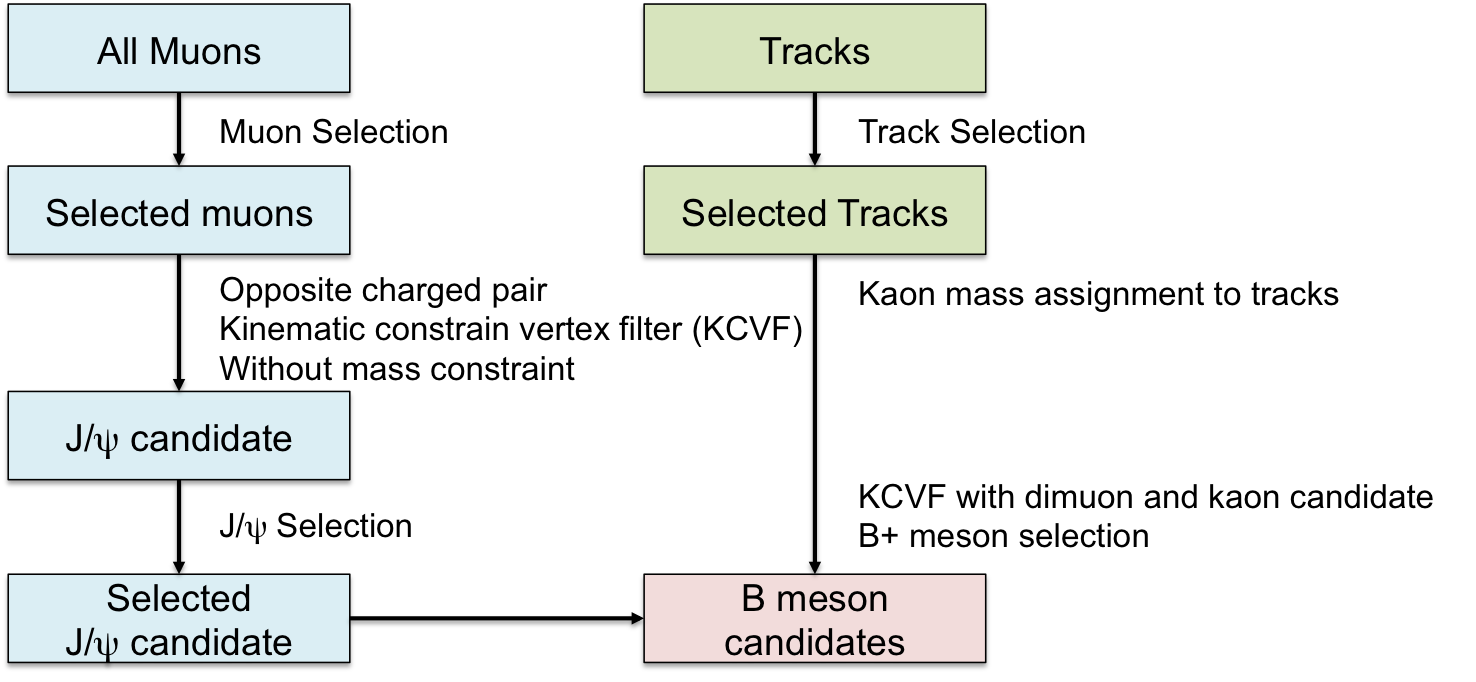
\includegraphics[width= 0.98\textwidth]{Figures/Chapter4/BPmesonWorkflow.png}
\caption{The schematic block diagram of the full reconstruction workflows for $B^+$ via the decay channel of $B^+ \rightarrow J/\psi K^+ \rightarrow \mu^+\mu^- K^+$ in the \textit{Bfinder} is shown above.}
\label{BPRECOWF}
\end{center}
\end{figure}

Here, we should note that since we do not have hadronic PID for the kaons, we assume the track to be kaons and assume the charged kaon PDG mass to the tracks \cite{AlphaTheoEx} to the tracks. Also, the invariant mass of muon pair is constrained to the nominal $J/\psi$ meson PDG mass ($m_{J/\psi}$ = 3.096916 GeV/c$^2$) \cite{AlphaTheoEx} instead of a distribution of the dimuon mass $m_{\mu\mu}$. The output file format of \textit{Bfinder} is an Ntuple. Each event will have multiple B-meson candidates \ref{BCand}.

\begin{figure}[h]
\begin{center}
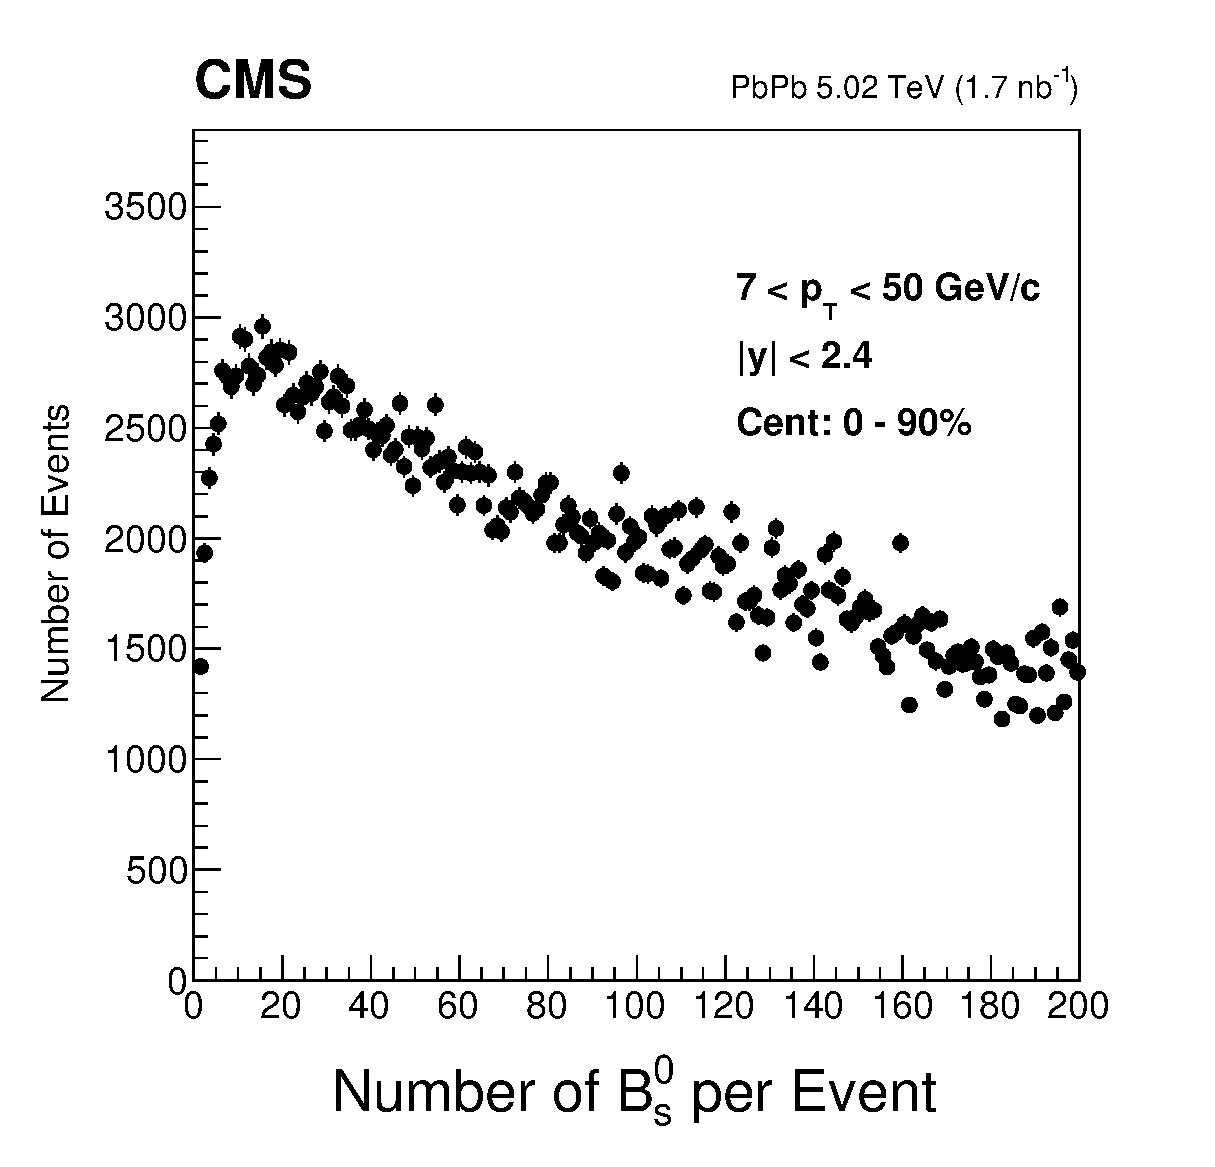
\includegraphics[width= 0.48\textwidth]{Figures/Chapter4/BsSize.eps}
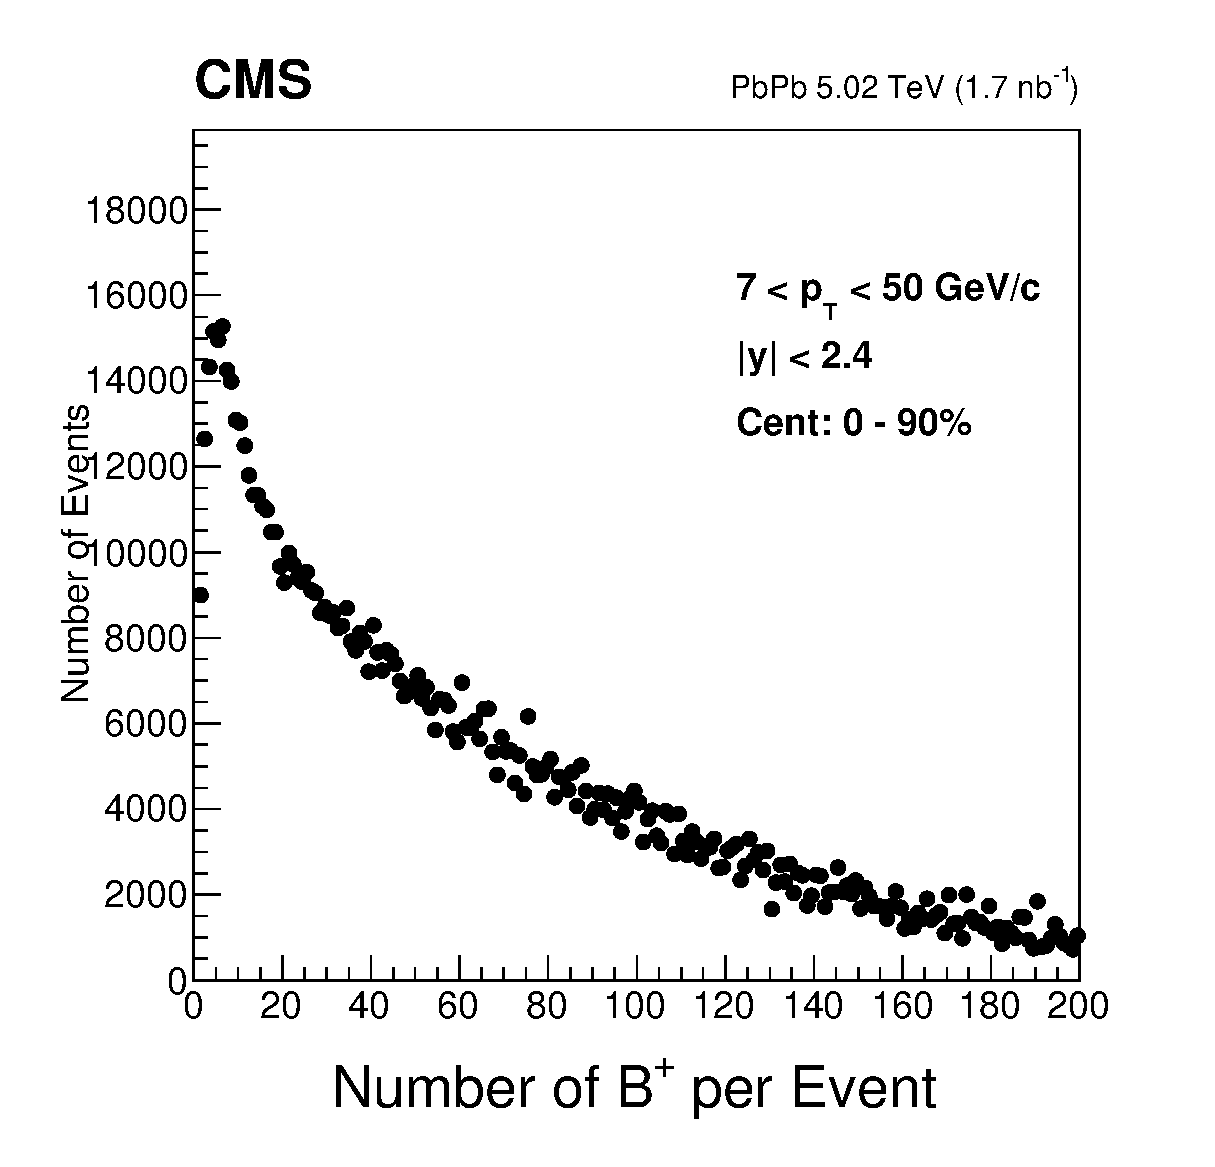
\includegraphics[width= 0.48\textwidth]{Figures/Chapter4/BPSize.eps}
\caption{The number of reconstructed B-meson candidates per event distribution in the dimuon PbPb data for $B^0_s$ (left) and $B^+$ (right) are shown above. Multiple B-meson candidates are reconstructed in one event.}
\label{BCand}
\end{center}
\end{figure}


Their information, including invariant mass, $p_T$, and $y$ as well as their daughter particles kinematics such as $p_T$ and $\eta$, is saved as a form of vector in each event. In this thesis, we use B-meson Ntuples to perform our analysis.


%\subsection{Decay Channels}


\subsection{Event Selections}

To ensure the quality of inelastic hadronic collisions events for B-meson reconstruct, we apply the follow selections


\begin{itemize}
\item At least one reconstructed primary interaction vertex, formed by two or more tracks
\item The longitudinal distance from the center of the nominal interaction region of less than 15 cm along the beam axis: $|$PV$_{z}$$| < $ 15
\item Compatible shapes of the clusters in the pixel detector with those expected from particles produced by a PbPb collision \cite{EvtSel}
\item At least two towers in each of the HF detectors with energy deposits of more than 4GeV per tower  
\end{itemize}

\subsection{Track Selections}

In addition to event selection, we also apply track selections to improve the quality of the tracks and reject fake tracks. For $B^+$ we have the following selections

\begin{itemize}
\item General Tracks passing high purity selection (describe in section 3.4.2)
\item $|\eta| < 2.4$ and $p_T > 1$ GeV/c
\item $p_T$ momentum resolution: $\frac{\sigma_{p_T}}{p_T} < 0.1$
\item At least 10 hits in the pixel + strip tracker layers: $N_{hit} > 10$
\item (Track $\chi^2/ndf$)/(pixel + strip hits) > 0.18
\item Vertex probability > 0.05
\end{itemize}

For $B^0_s$, since we expect it to have a $\phi$ resonance in the decay chain, we require the mass of the reconstructed dikaon candidate $|p_{K^+} + p_{K^-}| = m_{KK}$ to be 0.015 GeV/c$^2$ within the $\phi$ meson PDG mass ($m_\phi$ = 1.019455 GeV/c$^2$): $|m_{KK} - m_\phi| < 0.015$ GeV/c$^2$

\subsection{Muon Selections}

The muon candidates are selected according to the \textit{hybrid-soft muon} selection, developed for the muon analysis using CMS 2012 7 TeV $pp$ data \cite{SoftMuon}. It is adapted from the soft-muon ID developed in the BPH group, with two modifications: a) the purity selection is removed, and b) the muon is required to be also \textit{global}. This selection will be updated for the one developed in 2018. The \textit{hybrid-soft muon} selection includes the following cuts:


\begin{itemize}
\item Requirement to be Global Muon and Tracker Muon (described in section 3.4.3)
\item At least one good muons 
\item Transverse impact parameter $D_{xy}$ < 0.3 cm
\item Longitudinal impact parameter $D_{z}$ < 20 cm
\item At least 1 muon hits on pixel tracker layers and 5 hits on both the pixel + strip tracker layers 
\end{itemize}

In addition, an muon acceptance selection to ensure the muon candidate to have a total efficiency: $\epsilon^\mu > 10\%$. Table \ref{MuonAccCut} shows acceptance cuts, designed by the CMS muon analysis group, are also applied:

\begin{table}[h]
\begin{center}
\caption{Summary table of the muon acceptance selection for muon: $|\eta^\mu|$ as a function $p_T^\mu$.}
\vspace{1em}
\label{MuonAccCut}
  \begin{tabular}{ |c | c| c| c|}
    \hline 
Centrality &  $\langle N_{part} \rangle$ &$\langle N_{coll} \rangle$  & $\langle T_{AA} \rangle$  \\
     \hline
         \hline
 $|\eta^\mu|$ & 0 -- 1.2   & 1.2 -- 2.1  &  2.1 -- 2.4   \\
$p_T^\mu$ (GeV/c) &  > 3.5 &  > 5.47 - 1.89 & $\eta$  > 1.5   \\
     \hline
    \hline
\end{tabular}
\end{center}
\end{table}

Table \ref{MuonAccCut} comes from the muon analysis in the 2018 PbPb dataset. Figure \ref{MuonAccPlot} shows the muon reconstruction, identification, and trigger efficiency as a function of $p_T^\mu$ and $\eta^{\mu}$ \cite{MuonAccRef}

\begin{figure}[h]
\begin{center}
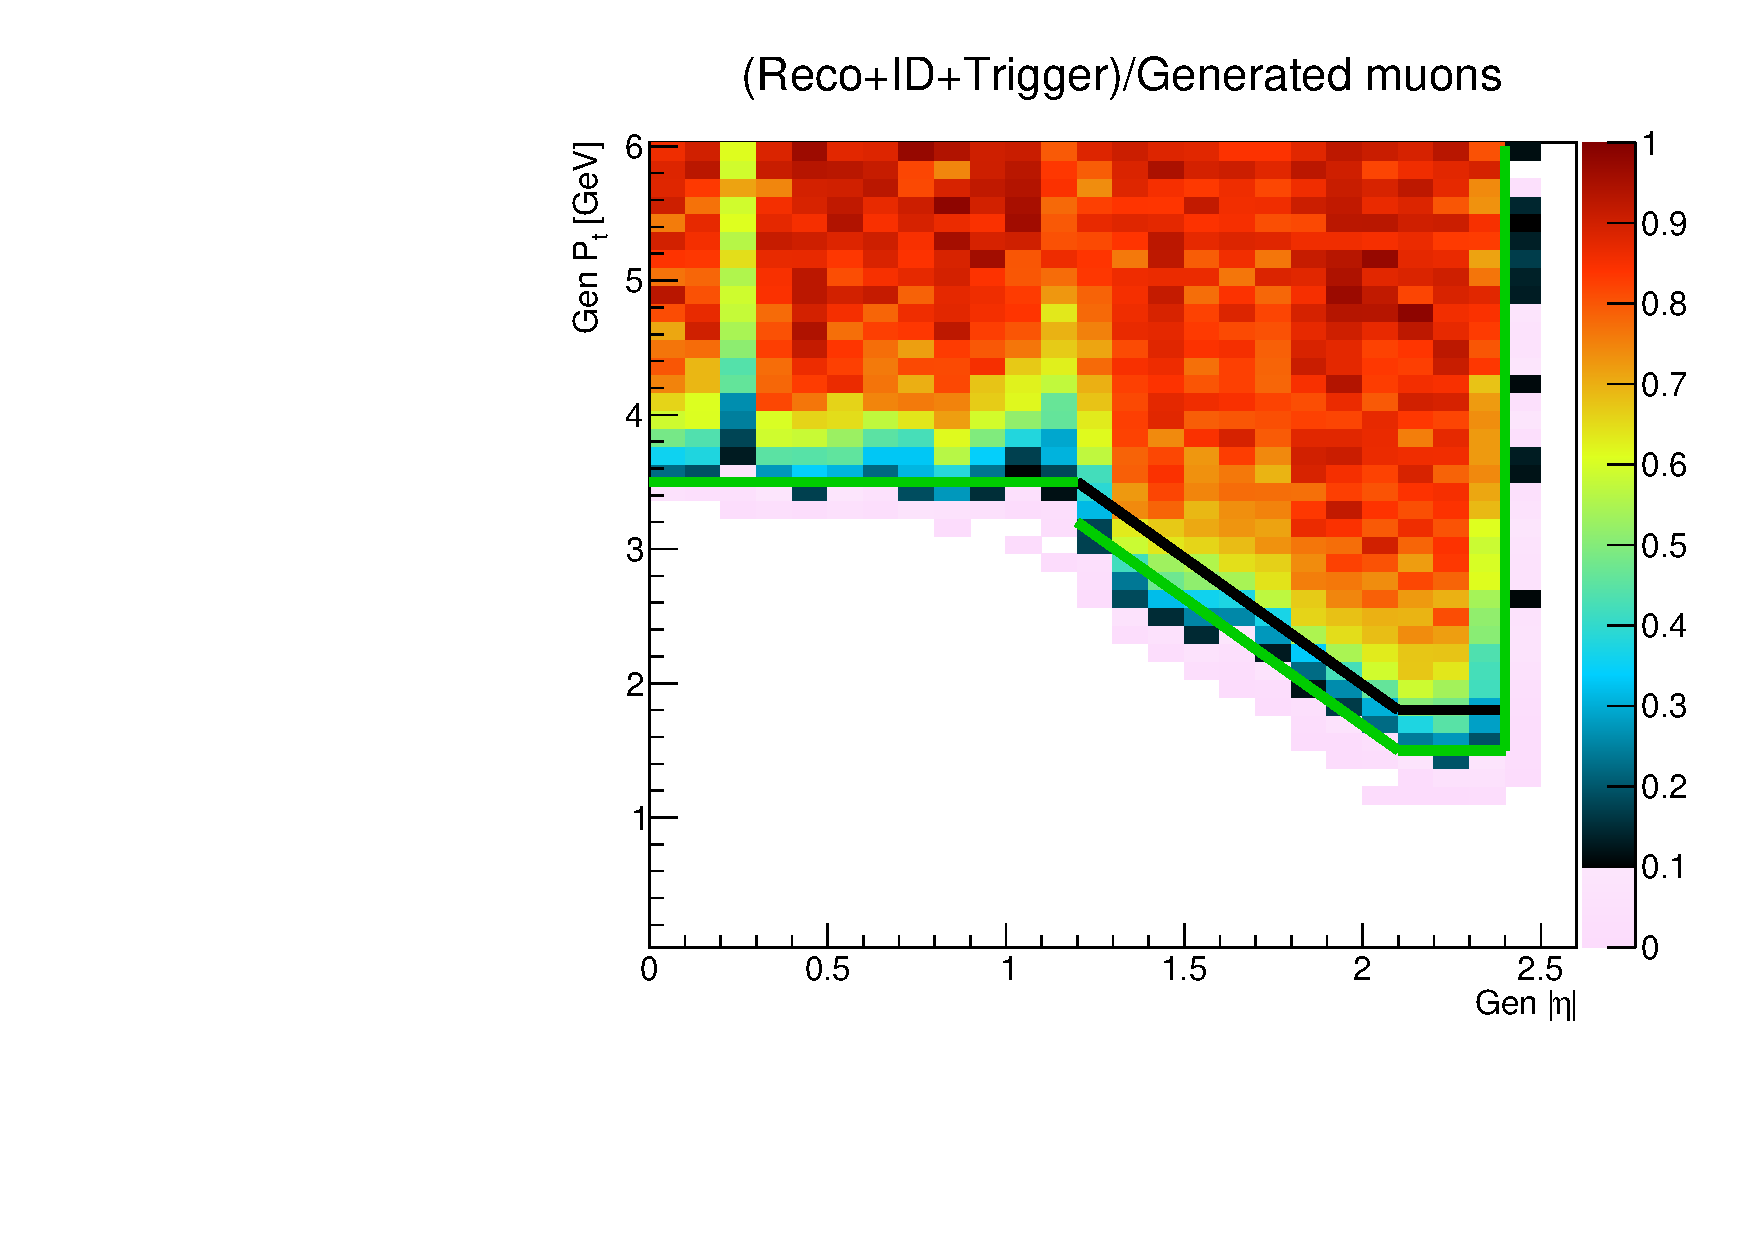
\includegraphics[width= 0.48\textwidth]{Figures/Chapter4/MuonAccPbPb.pdf}
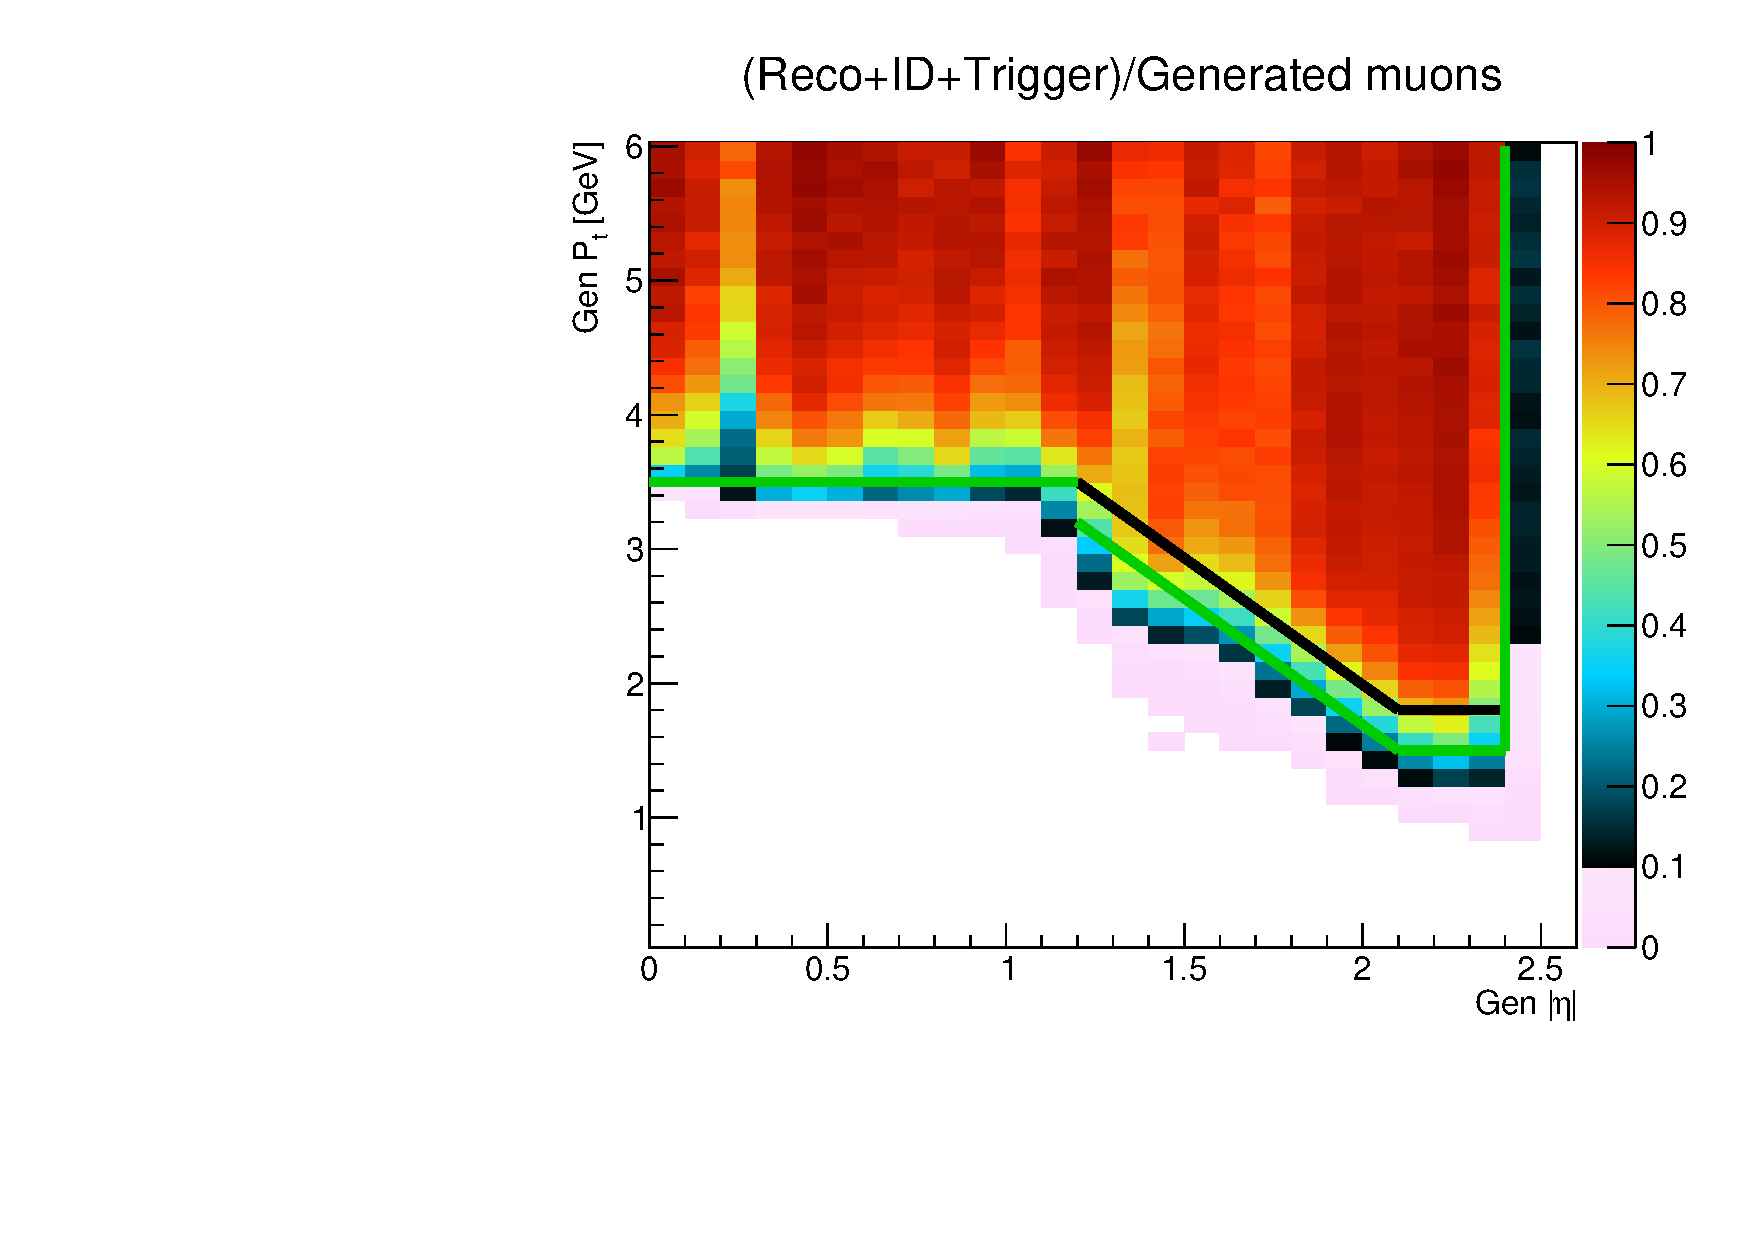
\includegraphics[width= 0.48\textwidth]{Figures/Chapter4/MuonAccPP.pdf}
\caption{The total efficiency, including reconstruction, identification, and trigger, of a single muon in 2018 PbPb (left) and 2017 pp (right) are shown above. The black curve is the 2015 PbPb and pp 90\% muon efficiency boundary while the green curve is the 2017 pp and 2018 PbPb 90\% muon efficiency boundary. The green boundary is translated to numerical values in Table \ref{MuonAccCut}}
\label{MuonAccPlot}
\end{center}
\end{figure}

We should note that there is a discontinuity of the muon acceptance selection at $|\eta| = 1.2$. Aside from the single muon selections, the following selections are applied to the reconstructed dimuon candidates


\begin{itemize}
\item Two muons have opposite charges 
\item Two mouns are tracker muons
\item Dimuon invariant mass about 0.15 GeV/c$^2$ near the $J/\psi$ PDG mass ($m_{J/\psi}$ = 3.096916 GeV/c$^2$): $|m_{\mu\mu} - m_{J/\psi}| < 0.15$ GeV/c$^2$
\item One muon is L2 muon and the other one is L3 muon (described in section 2.25)
\item Probability of the two muon tracks to originate from the same decay vertex $>$ 1\%
\end{itemize}

After applying all these preliminary selections to improve the quality of our dataset for the analysis, we are ready to perform cut optimization to further reject background candidates based on the decay topology of the $B^0_s$ and $B^+$ decay chains.


\section{Cut Optimization} 


Given the high combinatorial background, particularly in PbPb collision where we have thousands of tracks per event \cite{PbPbMulti}, it is not possible to observe B-meson resonance by simply applying the preselection presented in the previous section. Figure \ref{} shows the invariant mass distribution of fully reconstructed $B^0_s$ and $B^+$ at $7 < p_T < 50$ GeV/c after the event, track, and muon selections.

\begin{figure}[h]
\begin{center}
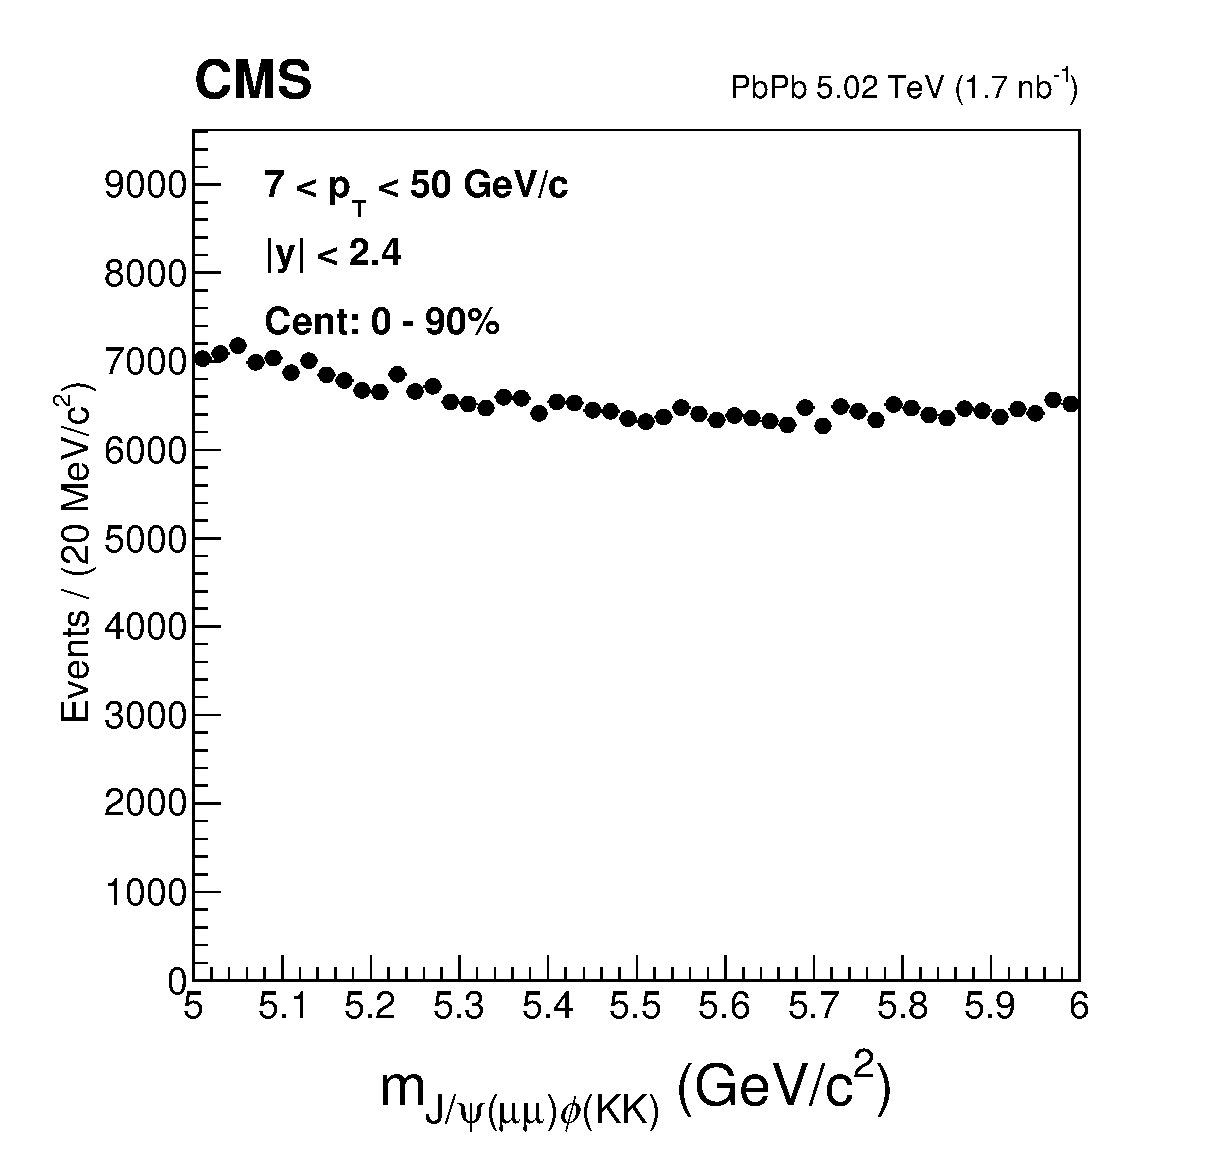
\includegraphics[width= 0.48\textwidth]{Figures/Chapter4/BsMassPreCut.eps}
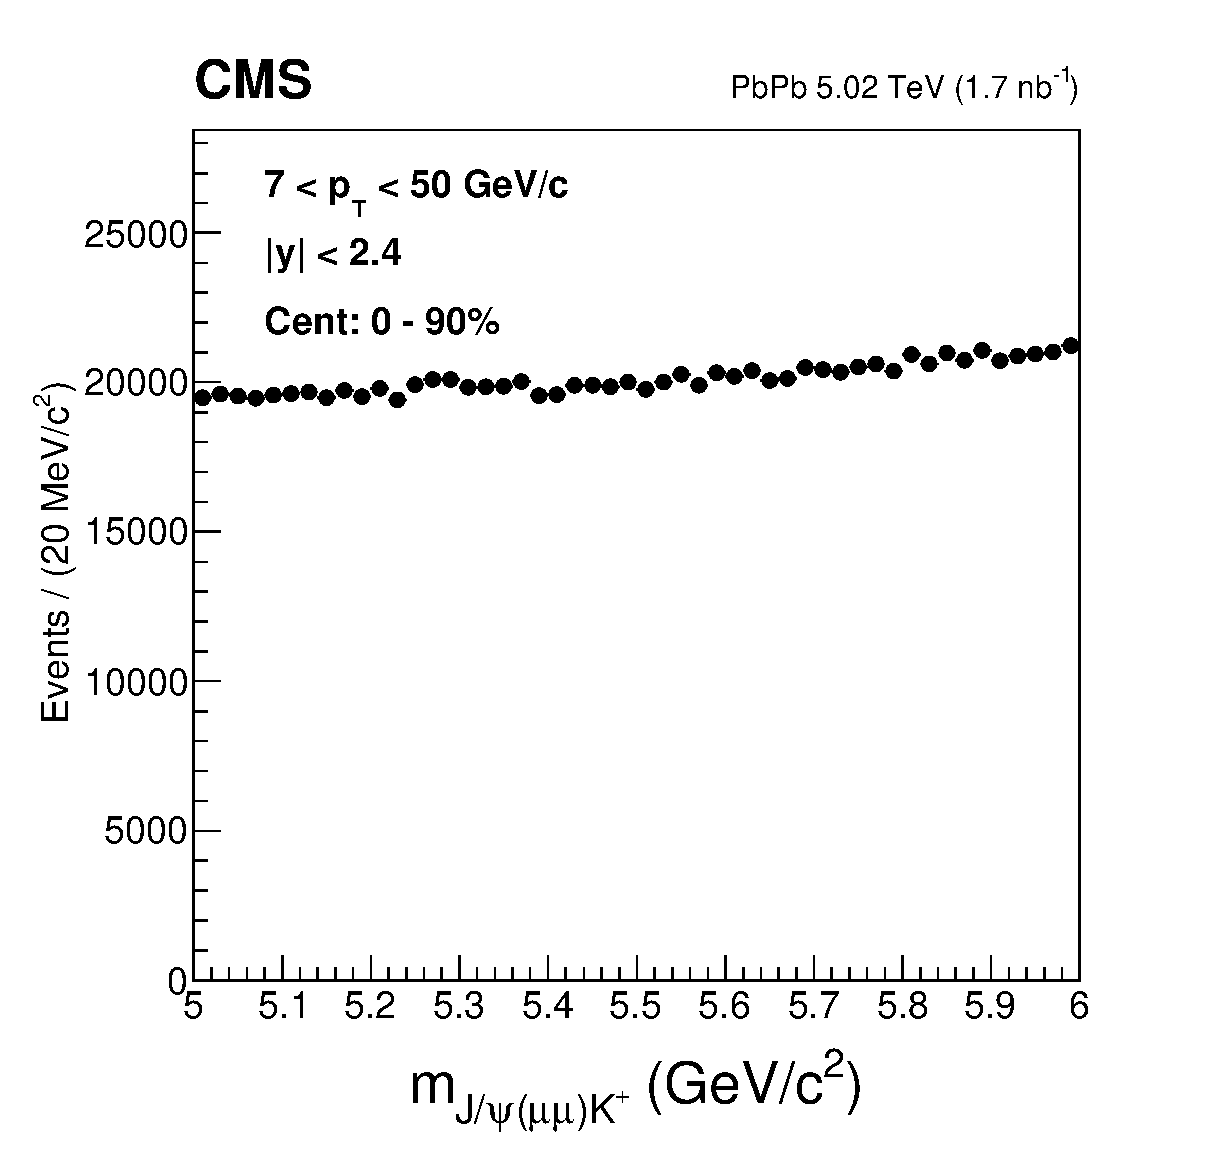
\includegraphics[width= 0.48\textwidth]{Figures/Chapter4/BPMassPreCut.eps}
\caption{The invariant mass distributions of fully reconstructed $B^0_s$ (left) and $B^+$ (right) after preselection are shown above.}
\label{MuonAccPlot}
\end{center}
\end{figure}


No B-meson signal is observed in the data. Therefore, aside from the preselections, a multivariate analysis (MVA) approach \cite{MVARef} is thus conducted in order to develop an optimal selection to separate signal B mesons from background and reconstruct a significant resonance in the invariant mass distribution in the data. The fitting performance is further related to both the amount of signal and background presented in the mass spectrum. 


\subsection{Topological Variables}


By an MVA analysis, one can then find the proper selection criteria which is optimized for this purpose. Several variables related to kaon tracks and B mesons decay topology are applied in order to reduce the combinatorial background that arises from random combination of tracks and muons. The topological variables used in B-meson analyses to be optimized by  are listed as follows:

\textbf{Topological Variables for $B^0_s$:}
\begin{itemize}
\item Kaon track $p_T$
\item Kaon track transverse distance to closest approach (DCA) significance: $DCA_{xy}/\sigma_{DCA_{xy}}$ 
\item Kaon track longitudinal distance to closest approach (DCA) significance: $DCA_{z}/\sigma_{DCA_{z}}$
\item Dikaon invariant mass distance to the $\phi$ meson PDG mass: $|m_{KK} - m_{\phi}|$
\item The $B^0_s$ meson decay length [or the distance between primary vertex (PV) and secondary vertex (SV)] significance: $|\vec{D}(SV,DV)|/|\sigma_{\vec{D}(SV,DV)}|$
\item The open angle between the B-meson decay length vector and its three momentum: $\alpha: \cos(\alpha) = \frac{\vec{D}(SV,DV) \cdot \vec{p}}{|\vec{D}(SV,DV)||\vec{p}|}$
\item The cosine angle of the opening angle in the transverse direction:  $\theta_B: \cos(\theta_B) = \frac{\vec{D(SV,DV)_{xy} \cdot \vec{p_T}}}{|\vec{D(SV,DV)_{xy}}||\vec{p_T}|}$
\item Vertex fitting probability: the $\chi^2$ value of the vertex fitting
\end{itemize}

For $B^+$, we also apply some addition rectangular selections before cut optimization

\textbf{Topological Variables for $B^+$:}
\begin{itemize}
\item Kaon track $p_T$
\item Kaon track $|\eta|$
\item Kaon track transverse distance to closest approach (DCA) significance: $DCA_{xy}/\sigma_{DCA_{xy}}$ 
\item The $B^+$ meson decay length [or the distance between primary vertex (PV) and secondary vertex (SV)] significance: $|\vec{D}(SV,DV)|/|\sigma_{\vec{D}(SV,DV)}|$
\item The open angle between the B-meson decay length vector and its three momentum: $\alpha: \cos(\alpha) = \frac{\vec{D}(SV,DV) \cdot \vec{p}}{|\vec{D}(SV,DV)||\vec{p}|}$
\item The cosine angle of the opening angle in the transverse direction:  $\theta_B: \cos(\theta_B) = \frac{\vec{D(SV,DV)_{xy} \cdot \vec{p_T}}}{|\vec{D(SV,DV)_{xy}}||\vec{p_T}|}$
\item Vertex fitting probability: the $\chi^2$ value of the vertex fitting
\end{itemize}

Figure \ref{DecayTopoBs} and \ref{DecayTopoBP} show the definition of topological variables of $B^0_s$ and $B^+$ decay chains respectfully 

\begin{figure}[h]
\begin{center}
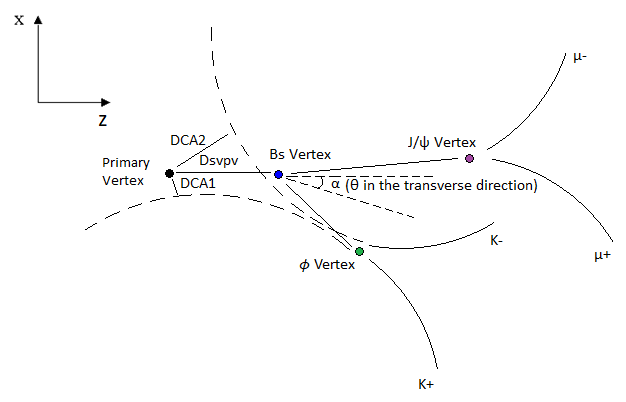
\includegraphics[width= 0.98\textwidth]{Figures/Chapter4/BsDecay.png}
\caption{The definition of topological variables in the decay of $B^0_s \rightarrow J/\psi \phi \rightarrow \mu^+\mu^- K^+K^-$ (left) are schematically shown above.}
\label{DecayTopoBs}
\end{center}
\end{figure}


\begin{figure}[h]
\begin{center}
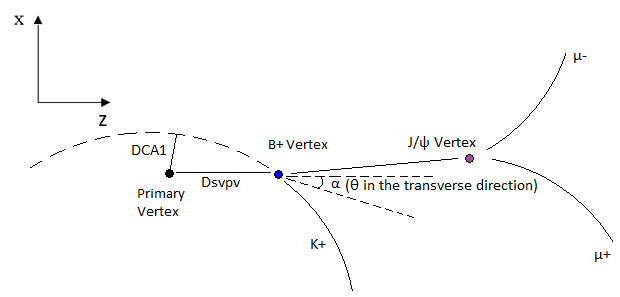
\includegraphics[width= 0.98\textwidth]{Figures/Chapter4/BPDecay.png}
\caption{The definition of topological variables in the decay of $B^+ \rightarrow J/\psi K^+ \rightarrow \mu^+\mu^- K^+ $ are schematically shown above.}
\label{DecayTopoBP}
\end{center}
\end{figure}

These topological variables will become the inputs to the multivariate analysis to optimize the signal significance.

\subsection{Multivariate Analysis}

In statistics, many data analysis techniques only focus on one or two variables individually. Multivariate analysis (MVA) analyzes more than two variables simultaneously to improve the data analysis. Figure \ref{MVADemo} shows schematically the advantages of MVA to traditional statistical techniques in data analysis to separate signal from background with two variables. 




\begin{figure}[h]
\begin{center}
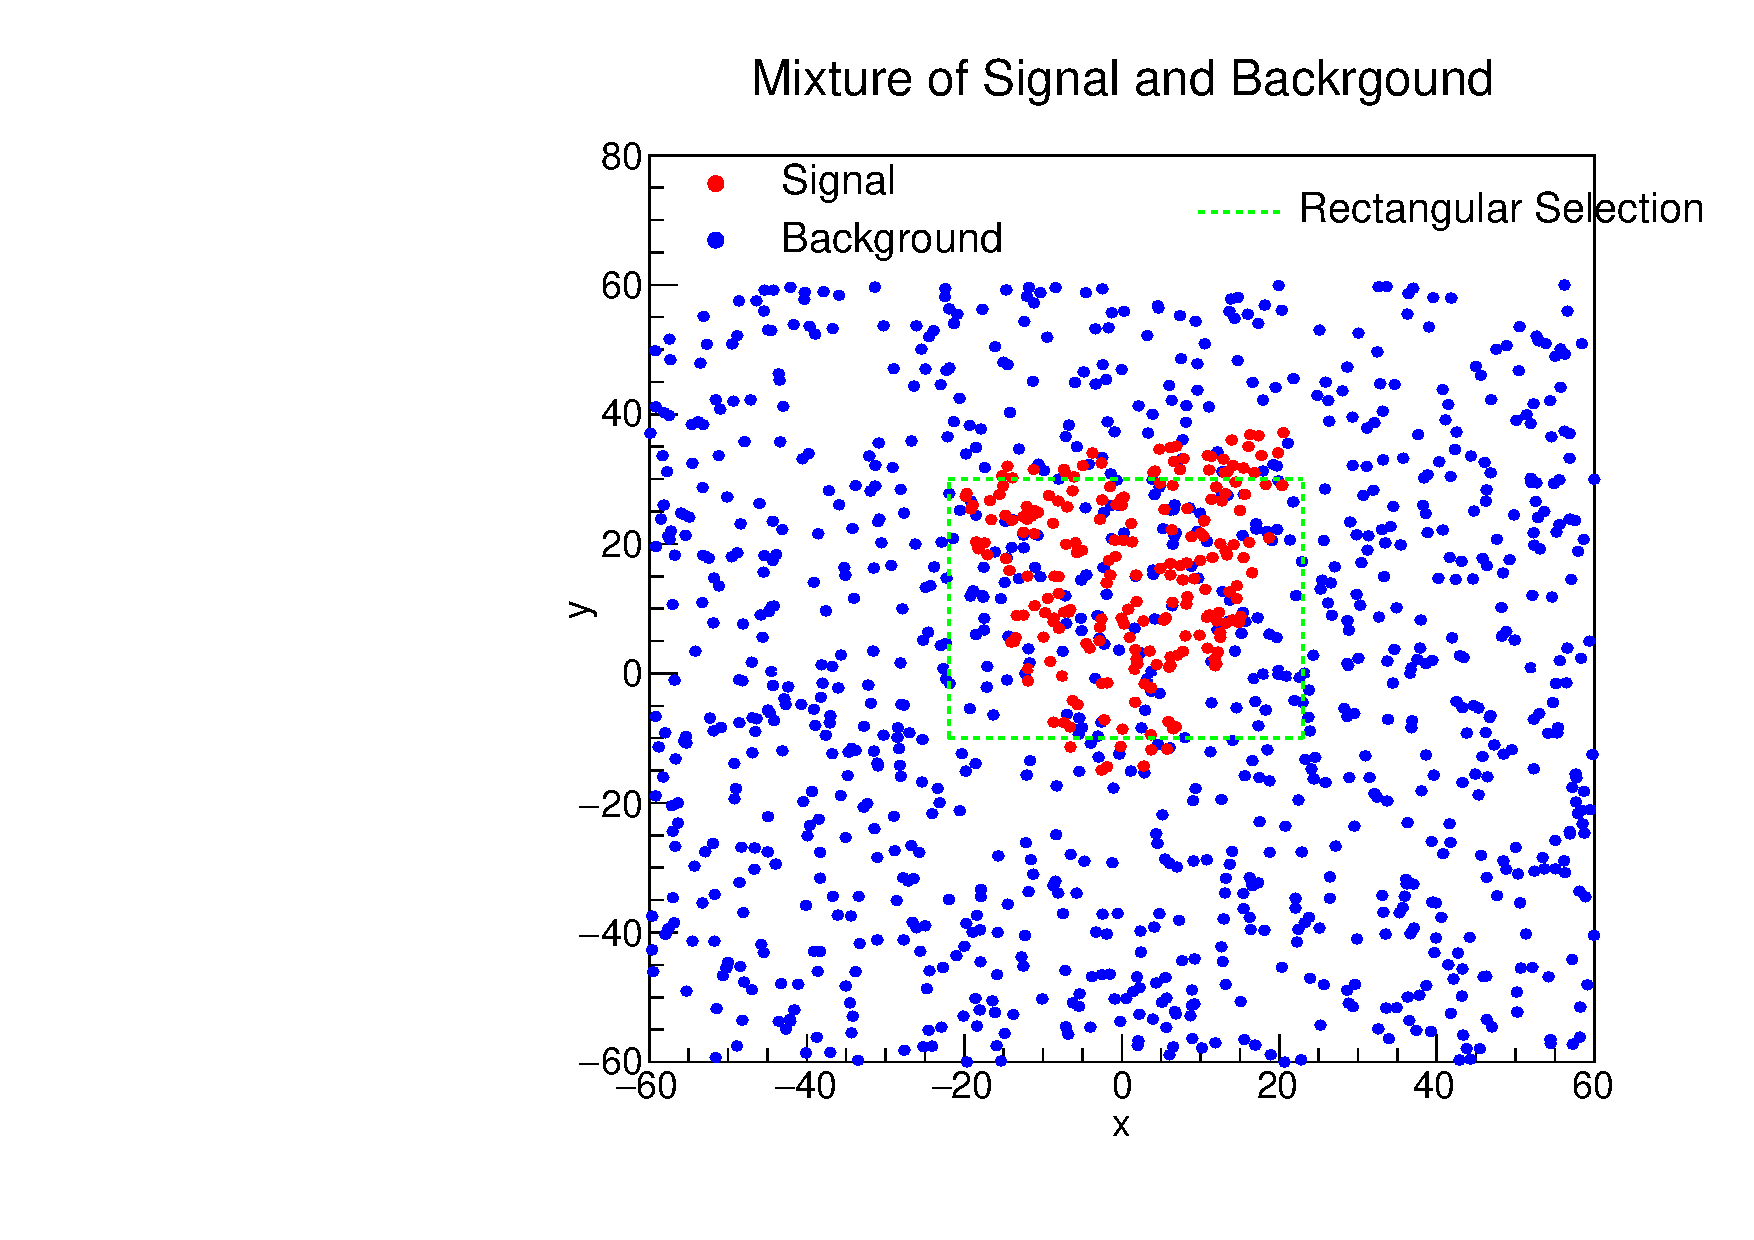
\includegraphics[width= 0.48\textwidth]{Figures/Chapter4/Rectangular.pdf}
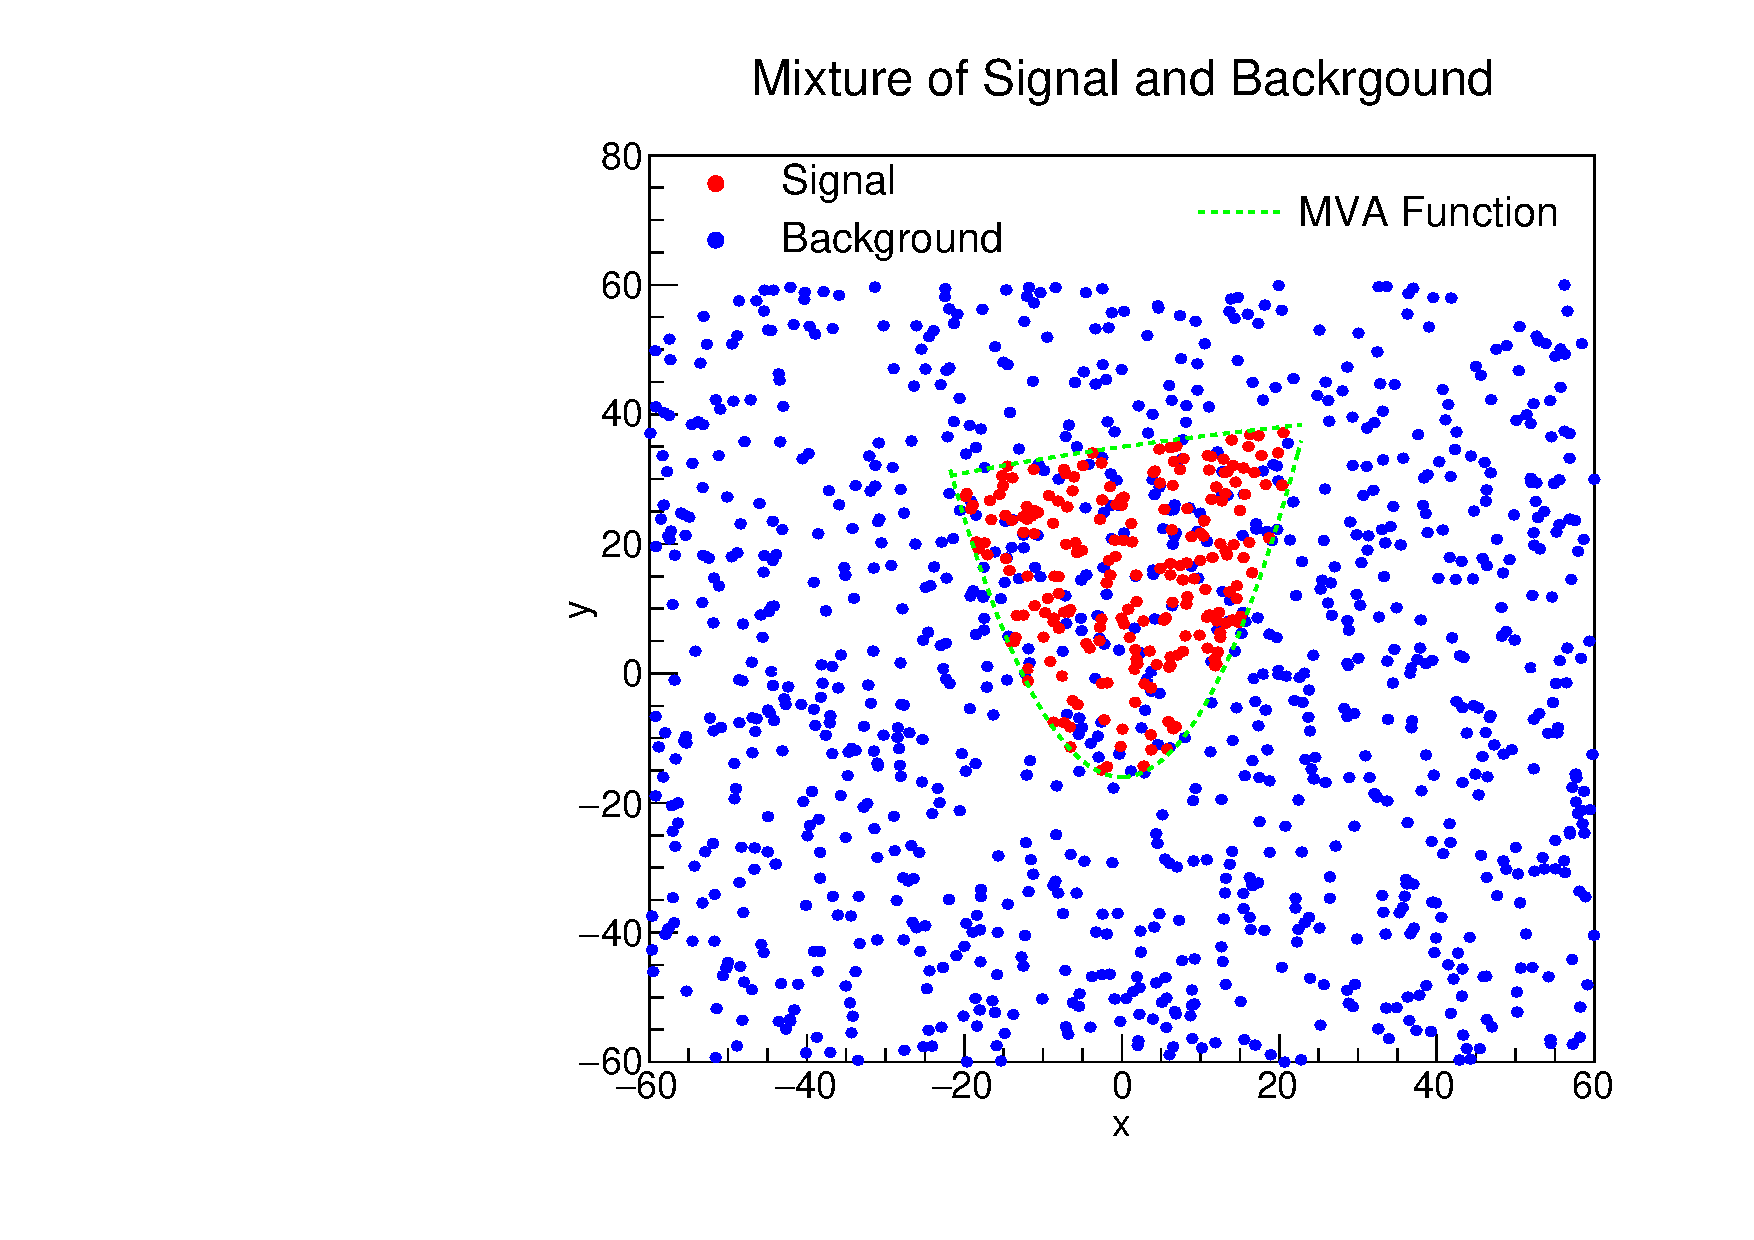
\includegraphics[width= 0.48\textwidth]{Figures/Chapter4/MVA.pdf}
\caption{The performance of traditional rectangular selection with a range of x and y (left) compared to the MVA method of a curve as a function of X and Y (right) are shown above. Here, we have the total signal S = 215 and the background B =  1000.}
\label{MVADemo}
\end{center}
\end{figure}

We can see that in multivariate analysis, an MVA value as a function of two independent variables $x$ and $y$: $MVA = f(x,y)$ is able to select signal out from background with higher purity (larger S/B ratio) than the rectangular selection function $x_1 < x < x_2$ and $y_1 < y < y_2$. Table \ref{MVAvsRec} shows the performance of MVA and traditional rectangular selections

\begin{table}[h]
\begin{center}
\caption{The comparison of the traditional rectangular selections to MVA for Figure \ref{MVADemo}.}
\vspace{1em}
\label{MVAvsRec}
  \begin{tabular}{ |c | c| c| c|}
    \hline 
Analysis Techniques &  S & B & S/B \\
     \hline
Rectangular & 174 & 135 & 1.29  \\
         \hline
MVA &   215  & 114  & 1.89  \\
     \hline
    \hline
\end{tabular}
\end{center}
\end{table}


\subsection{Machine Learning Techniques}

Machine learning, as branch of artificial intelligence, is the science that gets the computers to learn what human beings do. It is an automating data analysis method for model building to solve practical problems. Figure \ref{MLProblem} demonstrates the data analysis problems including classification, regression, and clustering, where machine learning could be applied.

\begin{figure}[h]
\begin{center}
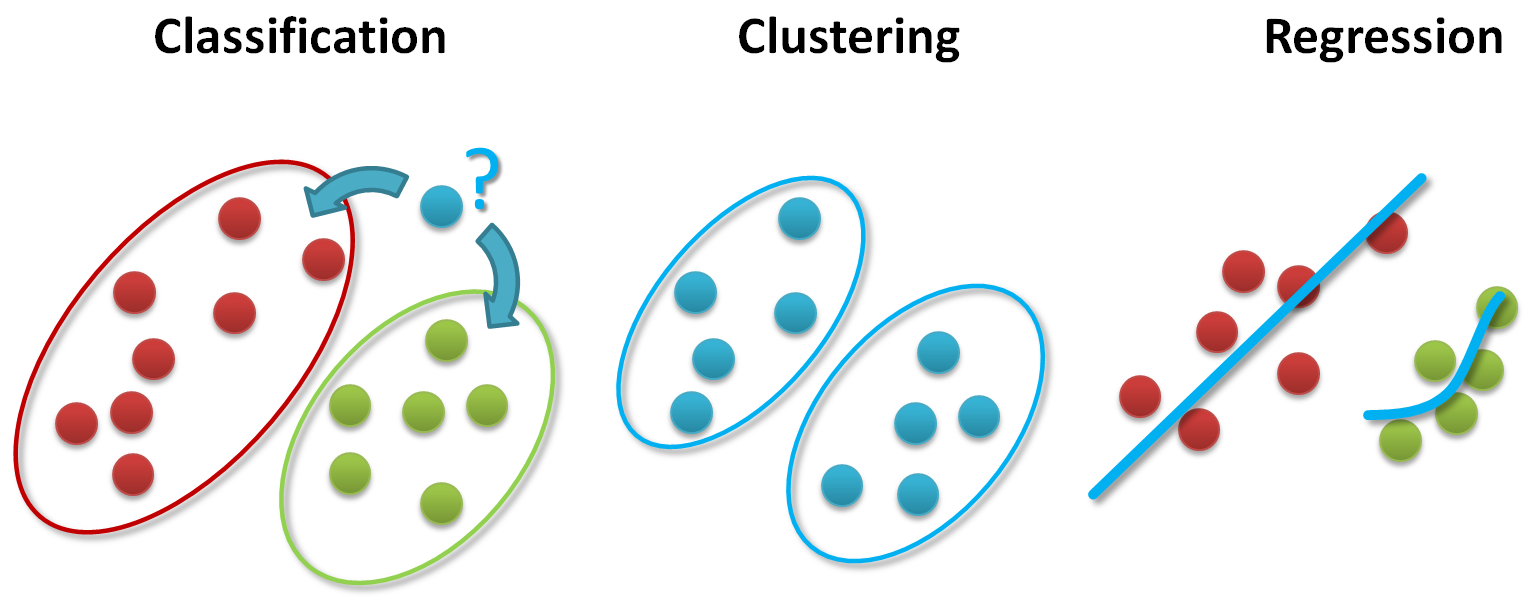
\includegraphics[width= 0.85\textwidth]{Figures/Chapter4/MLProblemsNew.png}
\caption{The solutions to classification, regression, and clustering problems with supervised and unsupervised machine learning approaches are shown schematically above.}
\label{MLProblem}
\end{center}
\end{figure}

In this analysis, our goal is to separate B meson signal out of the background. Therefore, it is a classification problem. Therefore, machine learning can be a power tool to solve our problems. We apply supervised machine learning to train the computer and let them find the optimal selections for B-meson analyses.   


\subsection{Terminologies}

The following list explains the technical jargons of machine learning techniques along with MVA that may be mentioned later in this thesis:


\begin{itemize}
\item \textbf{Training samples:} the input samples including both background and signal to train the computer. In this thesis, we use the B mesons candidates coming from our chosen B-meson decay channels (GEN Matched) in MC as the signal input and the B mesons candidates from the invariant mass sideband region with a distance of greater than 0.2 GeV/c$^{2}$ to the PDG mass of B mesons as background input to the \textit{TMVA} 
\item \textbf{Testing samples:} the samples including both background and signal going to be tested with the output from the training. The testing sample should not be the same as the training sample.
\item \textbf{Correlation matrix:} the linear correlation between the input variables for training 
\item \textbf{ROC curve:} the curve of signal efficiency as a function of the background rejection (= 1 $-$ background efficiency) for a given MVA value. Here the efficiency is defined as: efficiency = the number of candidates with the given MVA cut/ number of candidates without the MVA cut.
\item \textbf{Overtraining:} A Kolgomorgov test to compare the shape of the MVA distributions of training and test samples. It returns probabilities for both signal and background between 0 and 1. The closer to 0, the poor the matching, the more the overtraining will be.  
\end{itemize}




\subsection{Boosted Decision Tree Algorithm}

Nowadays, machining learning has become sophisticated. There are many well developed machining learning algorithms such as Rectangular Cut (CutsSA) Linear Discriminant (LD), Boosted Decision Tree (BDT), neutral network feed-forward Multilayer Perceptrons with recommended ANN with BFGS training method and bayesian regulator (MLPBNN), and Deep Learning in the market. Here, I will give a brief introduction about BDT algorithm in terms of \textit{Boosted} and \textit{Decision Tree}

\textbf{Boosted:} Boosted here refers to the ``boosting'' factor $\alpha$ in the hypothesis function to let the machine learn and correctly model the actual curve \cite{BoostingRef}. According to supervised machine learning, in order to use the boosting method, we first assign an ensemble of many weak learners (N) to create of a strong learner. The idea of boosting is to keep reweighing the function to enhance the classification and regression and performance by applying an MVA algorithm subsequently to the reweighed version of the training data in a sequential matter. Eventually, the hypothesis will converge a function that can describe the actual data. Figure \ref{Boosting} below shows schematically the boosting scheme 


\begin{figure}[h]
\begin{center}
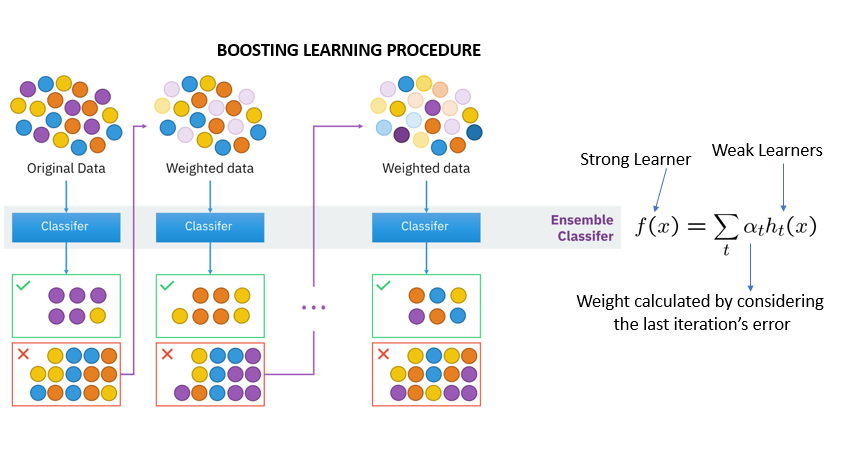
\includegraphics[width= 0.85\textwidth]{Figures/Chapter4/Boosting.jpg}
\caption{The schematic illustration of boosting procedures in machine learning is shown above.}
\label{Boosting}
\end{center}
\end{figure}


\textbf{Decision Tree:} A decision tree, sometime called as a regression tree, is a binary decision support tool using a tree-like model of decisions and list their possible consequences. Starting from a sampling to analyze, it sets up criteria for selections to decide the likelihood of signal and background based on the pure signal and background input samples. Then, it makes binary decisions (Yes/No), in each branch to select subset of samples out of the current sample, can be in sequentially or in parallel. It will then iterate multiple times until the sub samples are considered as signal or background. In TMVA machinery, the number of iteration is called \textit{NTree}. Figure \ref{DecisionTree} is a schematic demonstration of a decision tree with NTree = 4

\begin{figure}[h]
\begin{center}
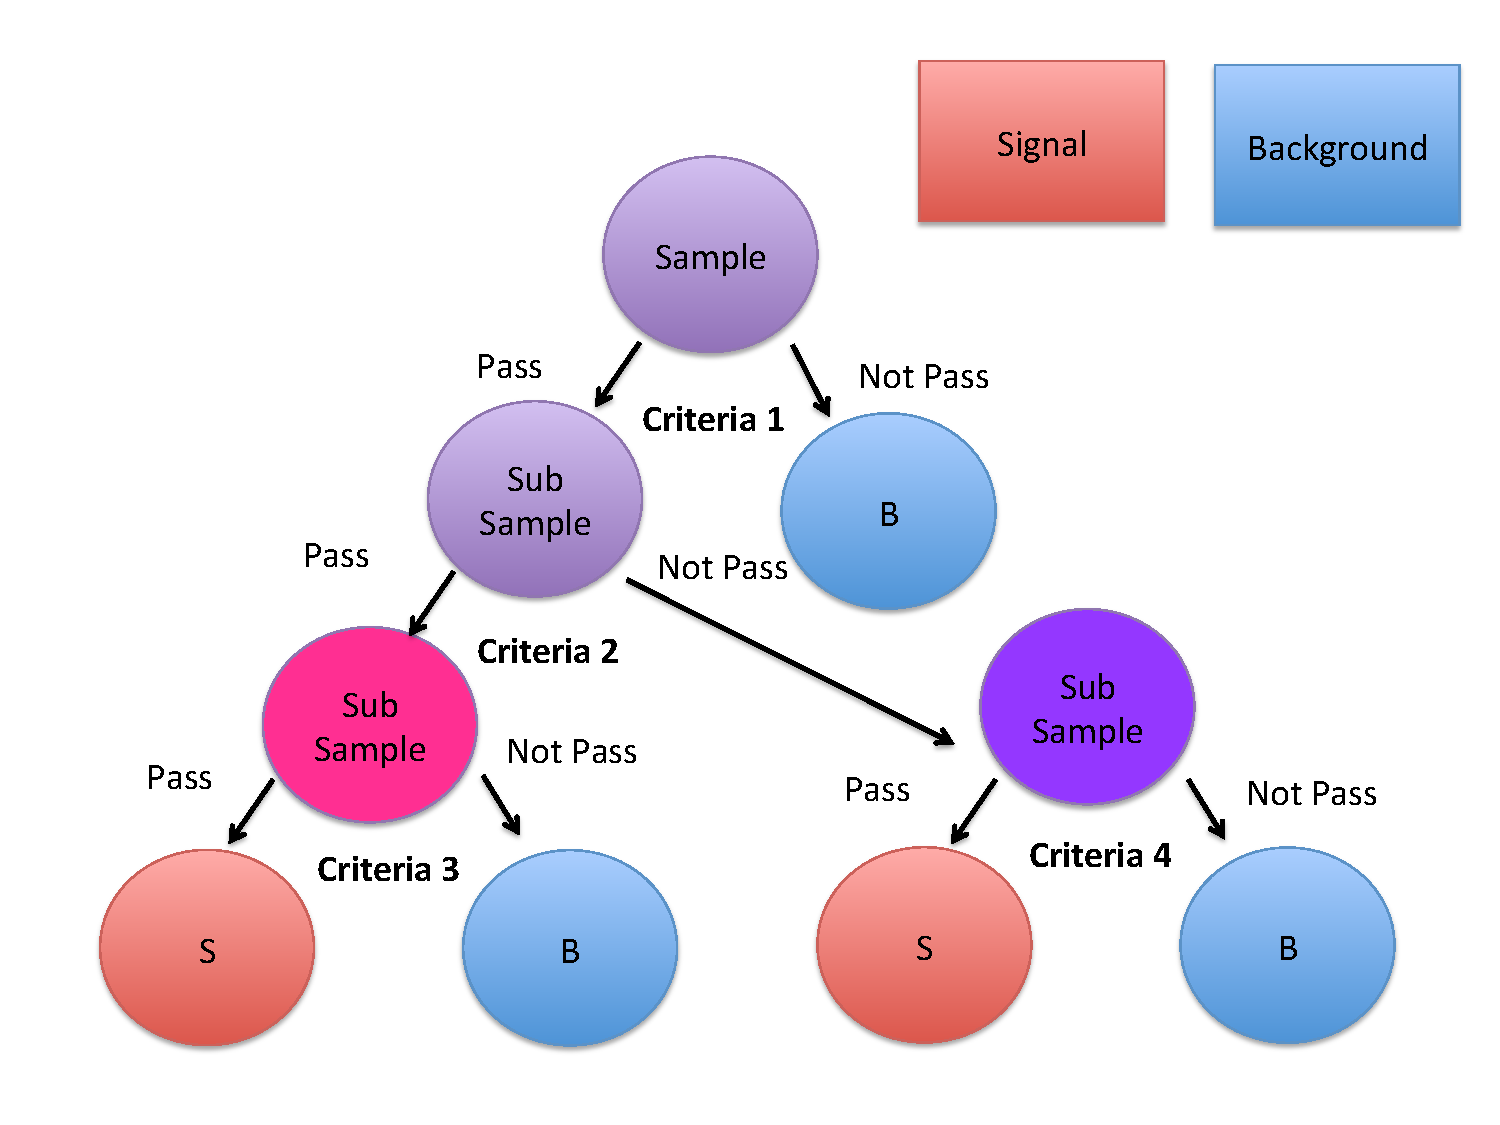
\includegraphics[width= 0.85\textwidth]{Figures/Chapter4/DecisionTree.pdf}
\caption{The schematic block diagram of a binary decision tree with NTree = 4 to separate signal and background in a training sample.}
\label{DecisionTree}
\end{center}
\end{figure}

In general, the performance of BDT will improve as NTree become larger. However, we should note that normally NTree is required to be smaller than the sample statistics. Otherwise, overtraining may occur and could induces bias in the data analysis.



\subsection{TMVA Training}


To perform machine learning, I use the Toolkit for Multivariate Data Analysis with ROOT (\textit{TMVA}) \cite{TMVA}, a dedicated ROOT base machine learning software framework on C++ programing language, to train the computer to find the optimal MVA value as a function of the topological variables in our B-meson analyses. We propose to optimize B mesons $p_T$ in the binning of [7, 10, 15, 20, 50] GeV/c individually. The following procedures are carried out:

Step 1: identify sufficient signal and background samples to train the computer within \textit{TMVA} machinery. 

Step 2: choose the training algorithms to use. Here, we choose CutsSA, CutsGA, BDT, MLP, and MLPBNN2 algorithms

Step 3: decide the training parameters for the each training algorithm. 

Step 4: run the TMVA machinery and generate the performance plots 

Step 5: choose the best algorithm according to the performance


\subsection{Training Performance}

After finishing the TMVA training procedure, we are ready to look at the training performance. First, we the correlation between the input topological variables. Figure \ref{CorrMatrix} shows the correlation matrices of $B^0_s$ and $B^+$ topological variables for B-meson $10 < p_T < 15$ GeV/c.

\begin{figure}[h]
\begin{center}
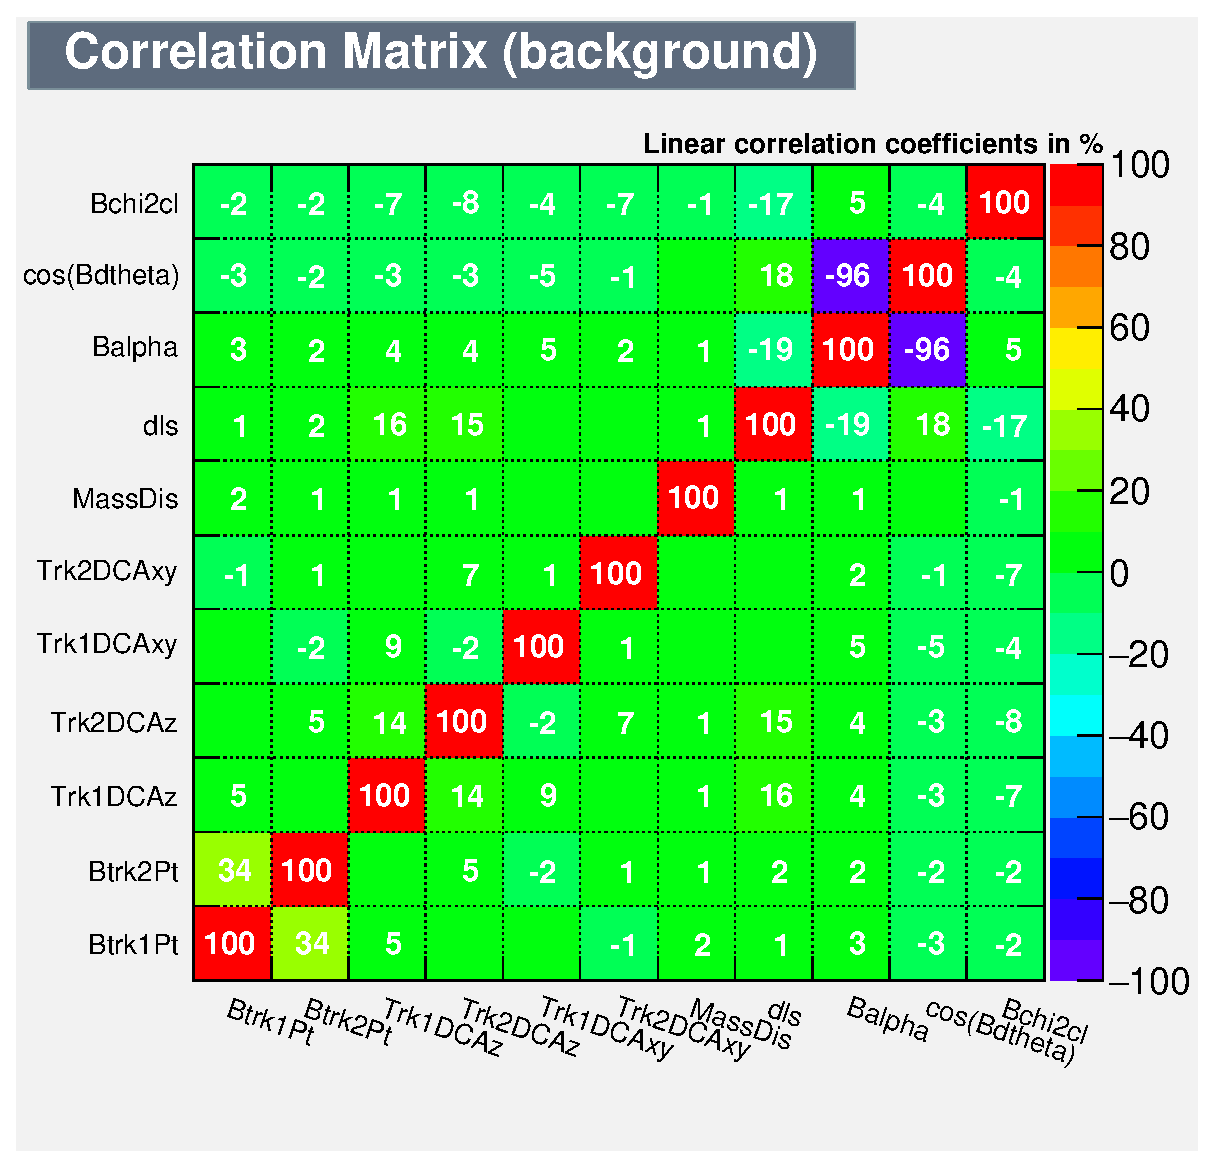
\includegraphics[width= 0.48\textwidth]{Figures/Chapter4/BsCorr_10_15.eps}
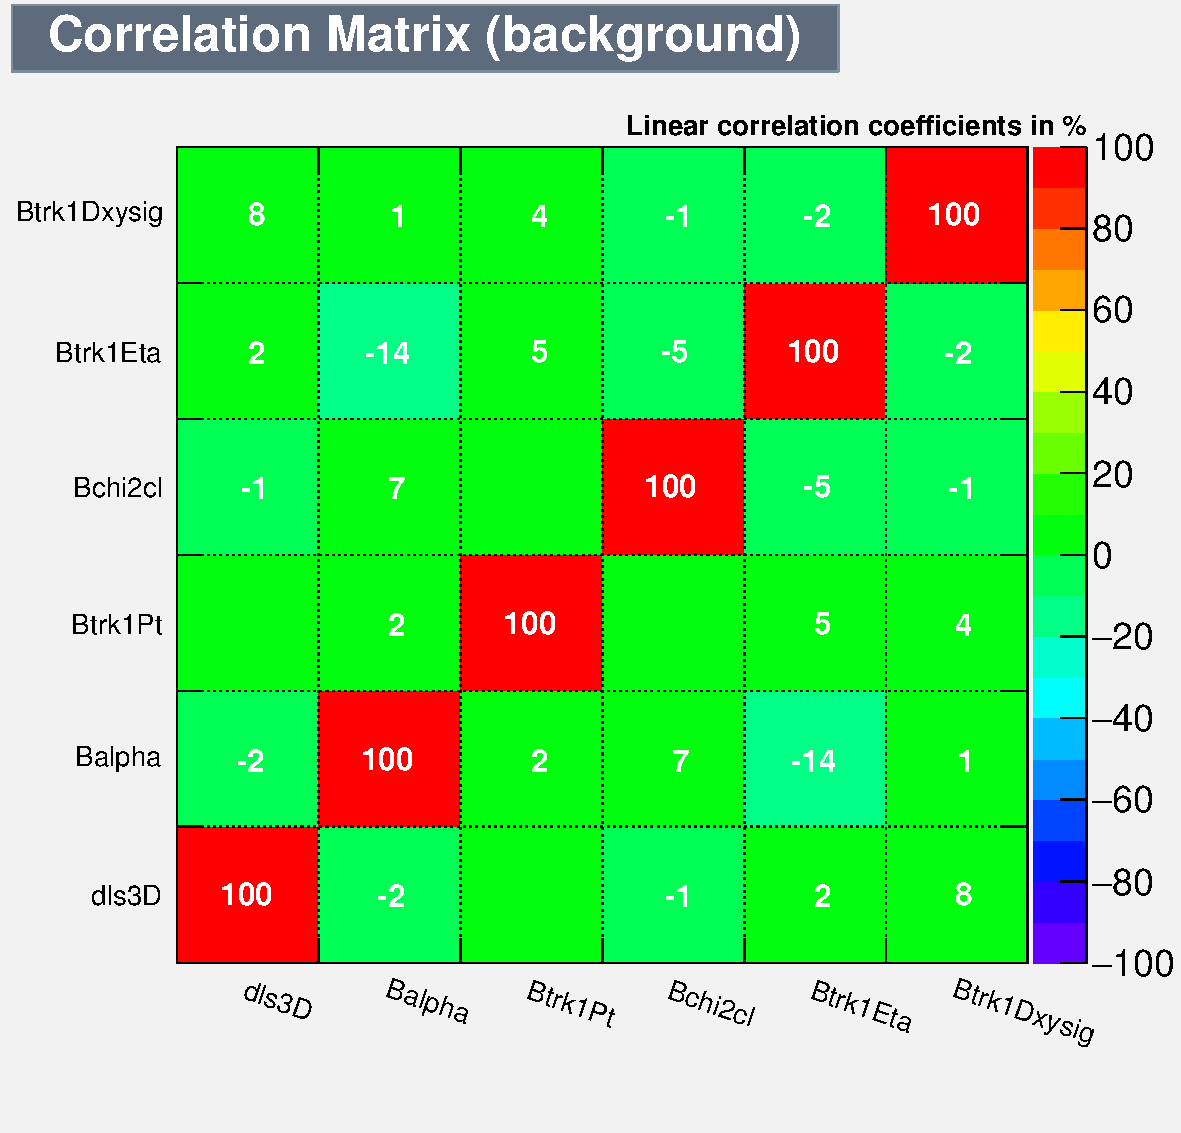
\includegraphics[width= 0.48\textwidth]{Figures/Chapter4/BPCorr_10_15.pdf}
\caption{The correlation matrices of $B^0_s$ (left) and $B^+$ (right) in data at $10 < p_T < 15$ GeV/c are shown above.}
\label{CorrMatrix}
\end{center}
\end{figure}

We can see that there are no significant correlation among the topological variables except the open angle $\alpha$ and the cosine its transverse projection $ \cos\theta$, which is know. Therefore, the variable sets we input to the \text{TMVA} training are good.  

Next we compare the overall performance among the algorithms. Figure \ref{ROCAll} below shows the ROC curves for $B^0_s$ \textit{TMVA} training at 10 $< p_T < $ 15 GeV/c.

\begin{figure}[h]
\begin{center}
\includegraphics[width= 0.80\textwidth]{Figures/Chapter4/BsROC.png}
\caption{The $B^0_s$ ROC curves of CutsSA, CutsGA, BDT, MLP, and MLPBNN2 algorithms are shown above.}
\label{ROCAll}
\end{center}
\end{figure}

We should note that the number of tree for BDT here is NTree = 2000. From Figure \ref{ROCAll}, we can see that BDT has the best performance compared to other algorithms in the given parameter settings. Basically, for a given background rejection, the BDT curve has the highest signal efficiency. It is closer to the upper right corner, which is the perfect algorithm. Therefore, we decide to use BDT algorithm to look for the optimal selections in all $p_T$ bins in both $B^0_s$ and $B^+$ analysis.


Finally, before, implementing the BDT algorithm to the analysis, we also check the overtraining and make sure that no significant overtraining is observed. Figure \ref{OverTraining} show the overtraining test for both $B^0_s$ and $B^+$ BDT at 10 $< p_T < $ 15 GeV/c. 


\begin{figure}[h]
\begin{center}
\includegraphics[width= 0.48\textwidth]{Figures/Chapter4/BsOT.png}
\caption{The $B^0_s$ ROC curves of CutsSA, CutsGA, BDT, MLP, and MLPBNN2 algorithms are shown above.}
\label{ROCAll}
\end{center}
\end{figure}

According to Figure \ref{OverTraining}, neither signal nor background of $B^0_s$ and $B^+$ BDT is vanishing. Hence, no significant overtraining is observed. The BDT trainings are valid to use in the $B^0_s$ and $B^+$ analysis.


\subsection{Working Point Determination}

Now with the BDT training results, next step is to choose the BDT selection that can give us the best analysis results. Next step working point chose avoid bias


\subsection{Selection Performance}

To check the performance BDT selections, we look at the dimuon and dikaon invariant mass distributions to see if $J/\psi$ and $\phi$ resonance are observed. Figure \ref{mesonpeakPbPb} shows the after apply the selections


\begin{figure}[h]
\begin{center}
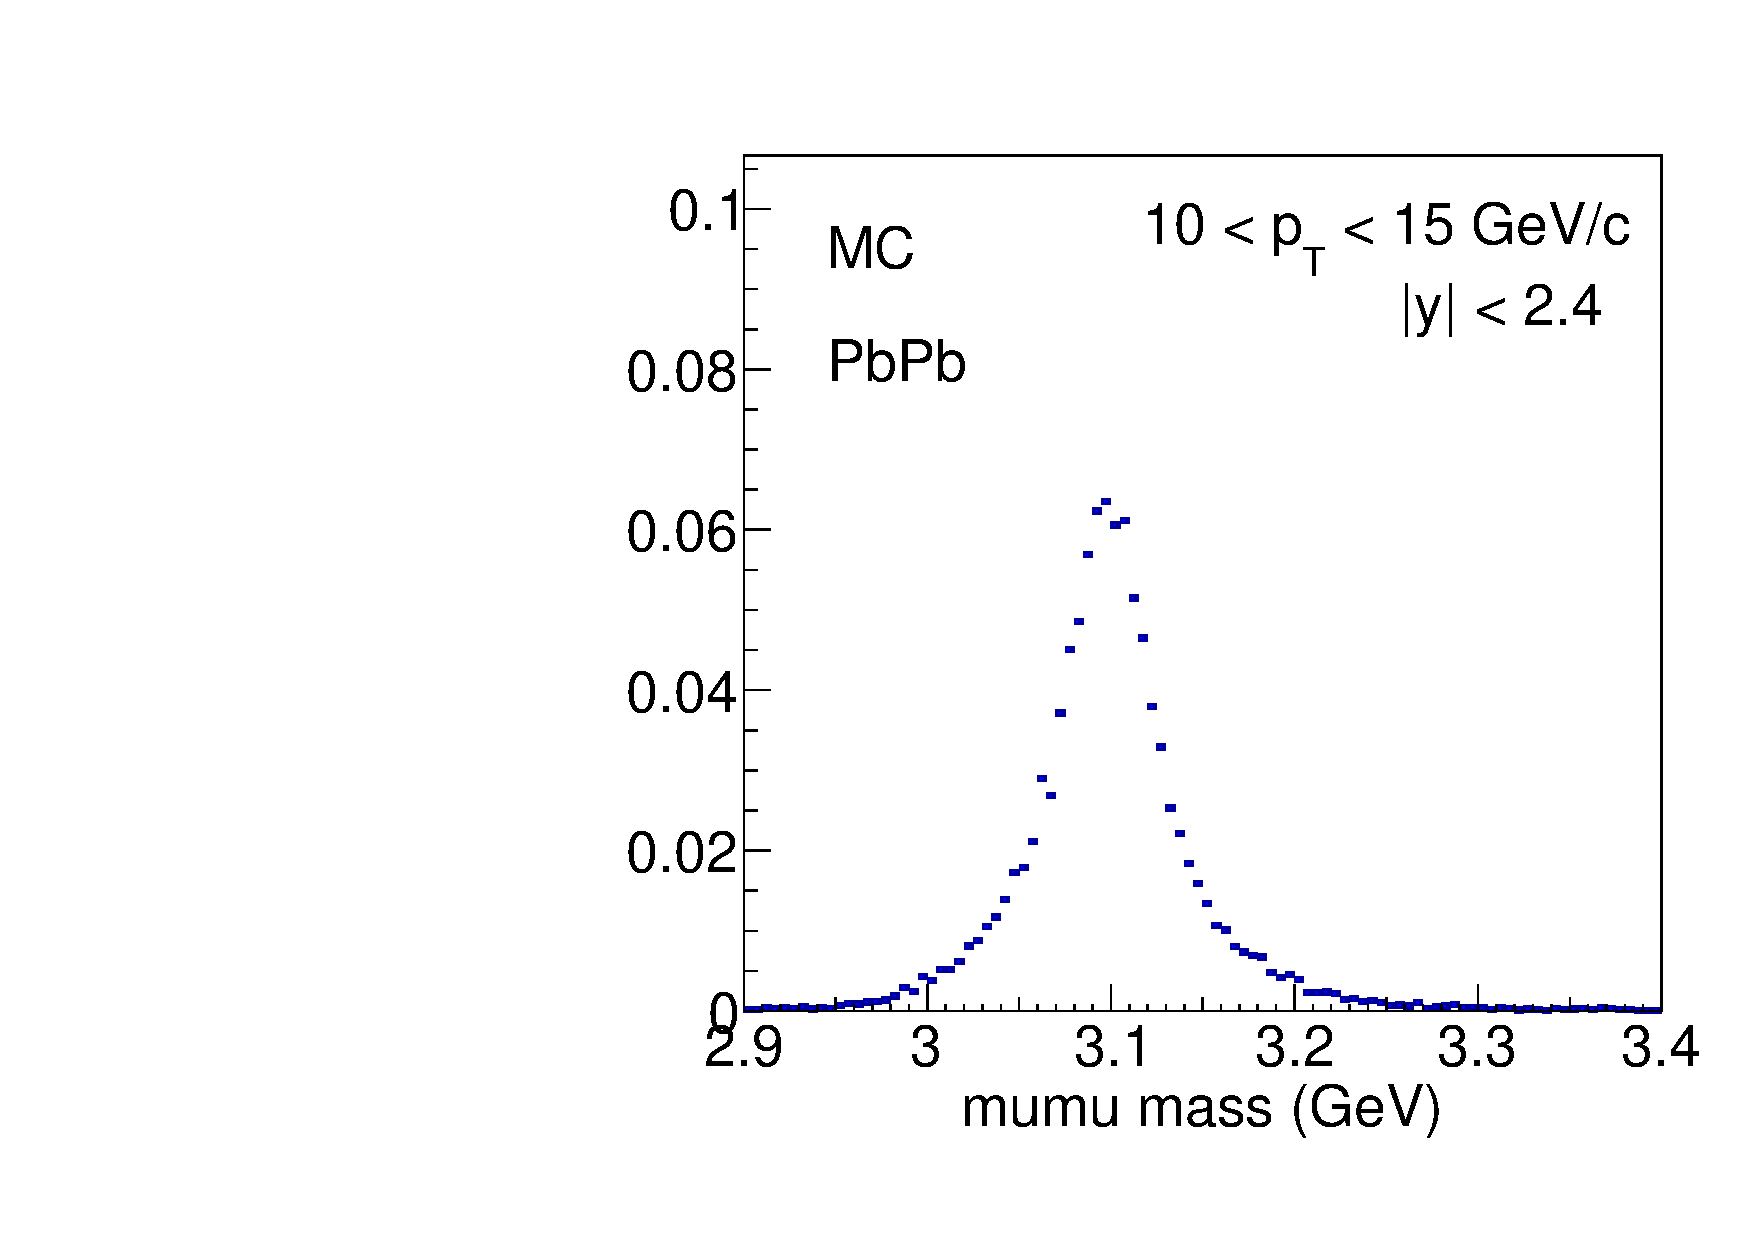
\includegraphics[width=0.42\textwidth]{Figures/Chapter4/mc_PbPb_1_Bmumumass.pdf}
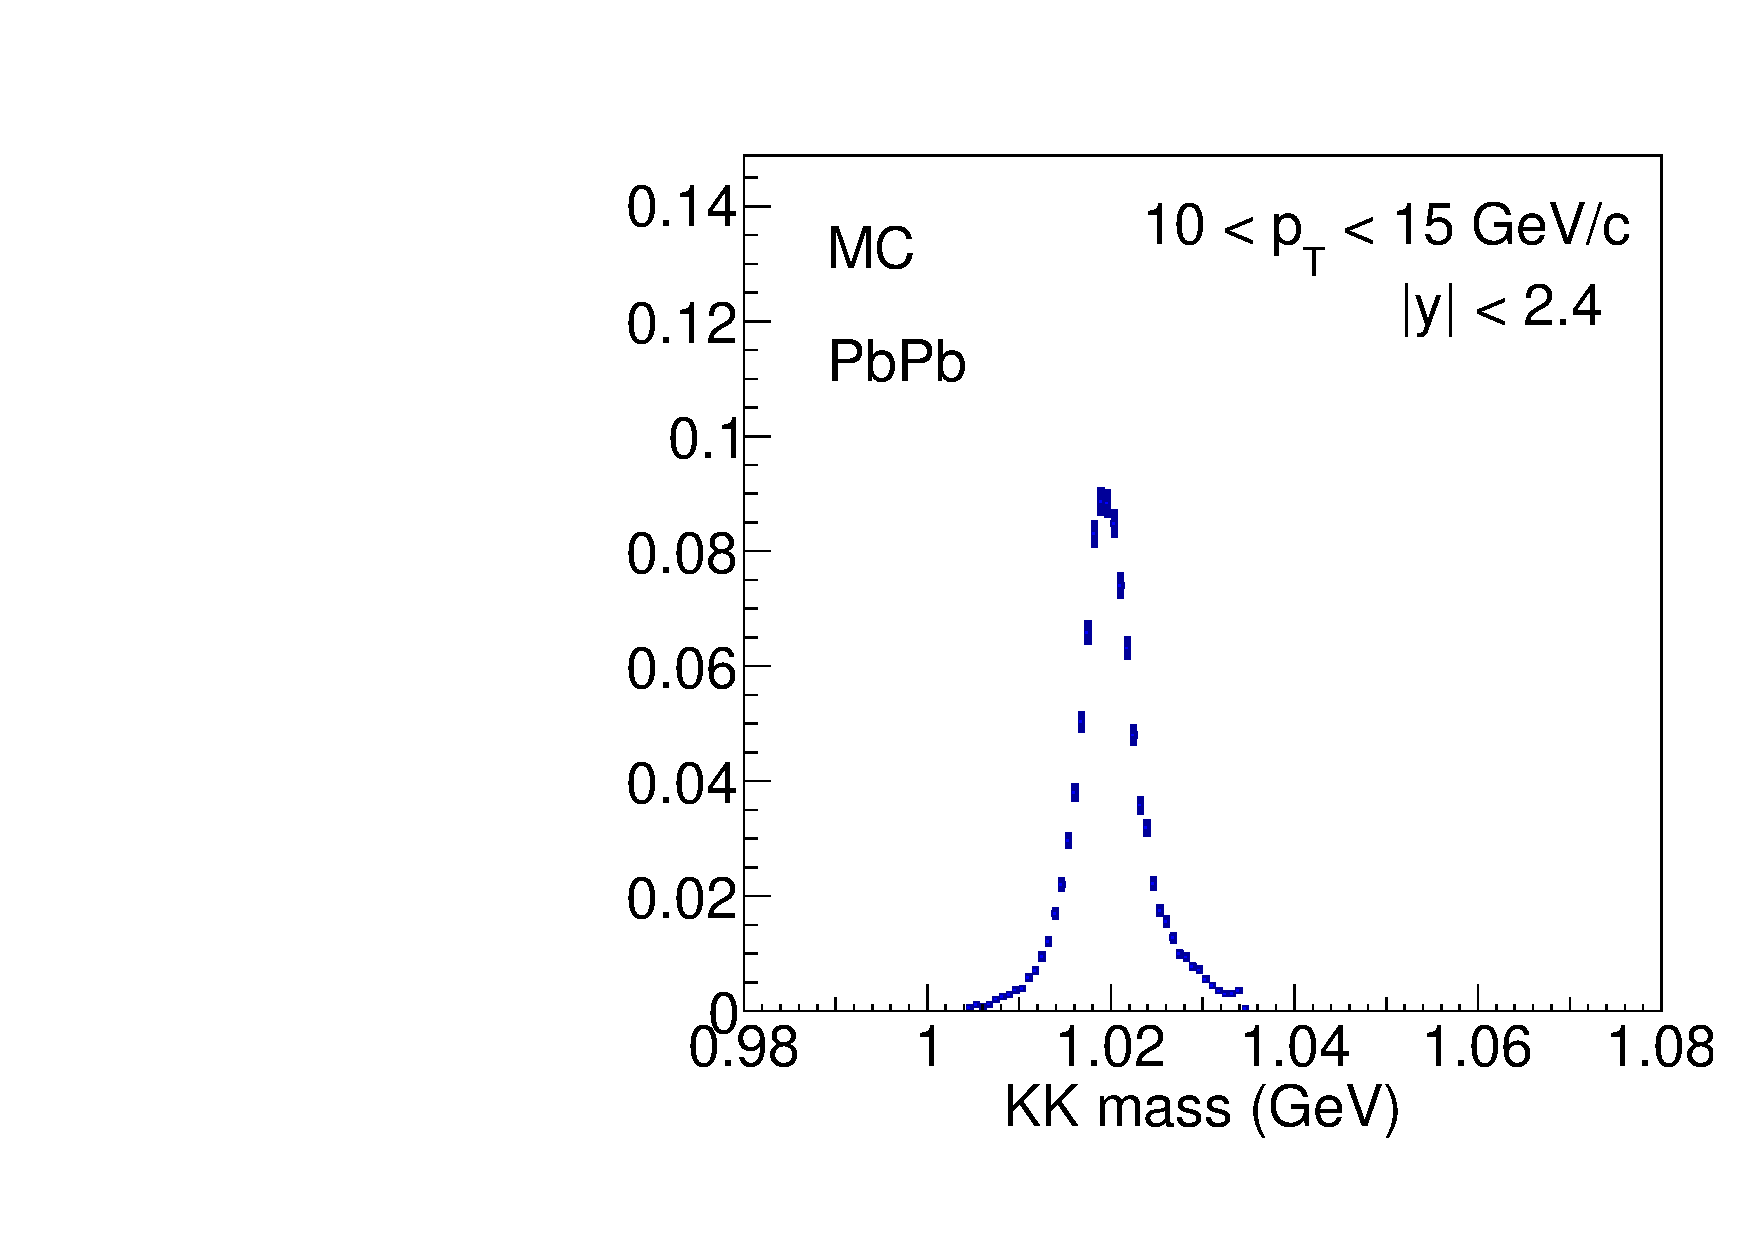
\includegraphics[width=0.42\textwidth]{Figures/Chapter4/mc_PbPb_1_Btktkmass.pdf}
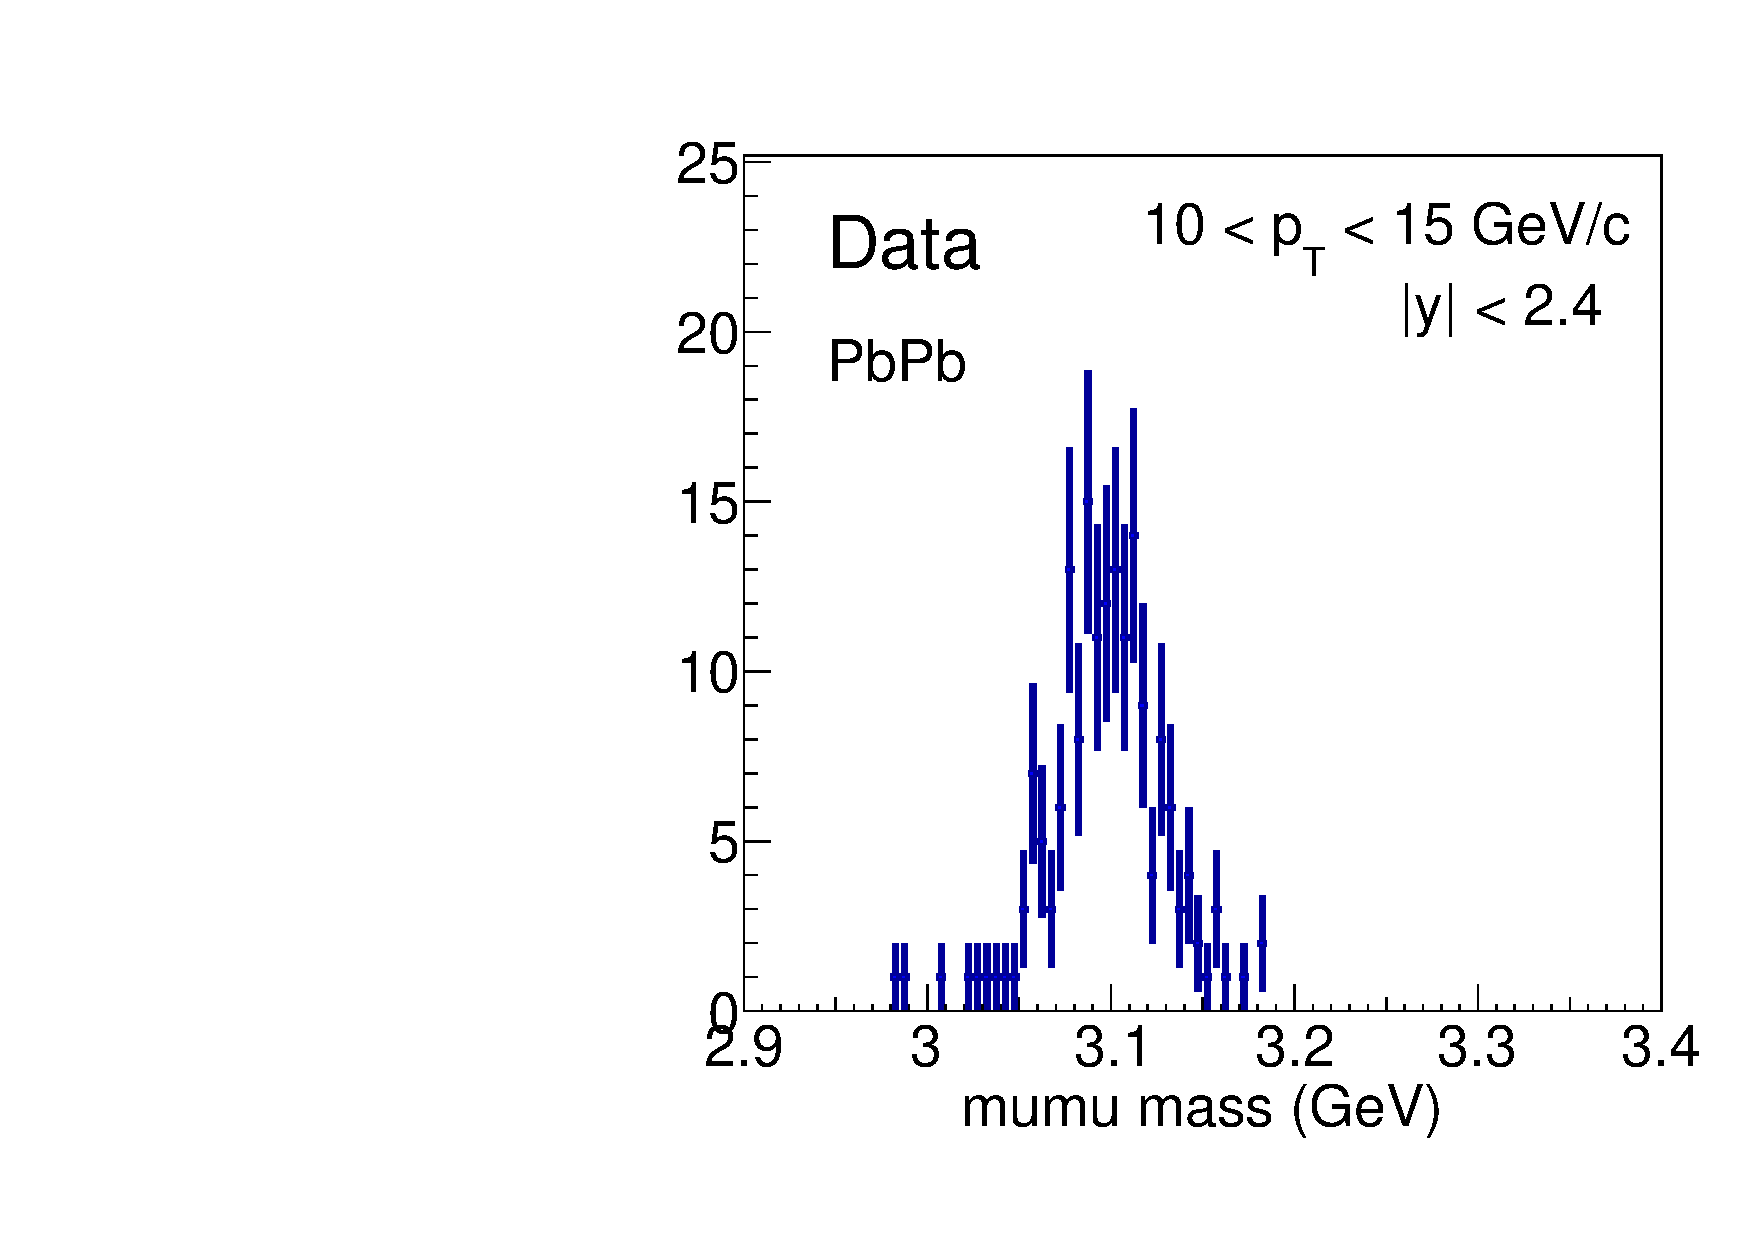
\includegraphics[width=0.42\textwidth]{Figures/Chapter4/data_PbPb_1_Bmumumass.pdf}
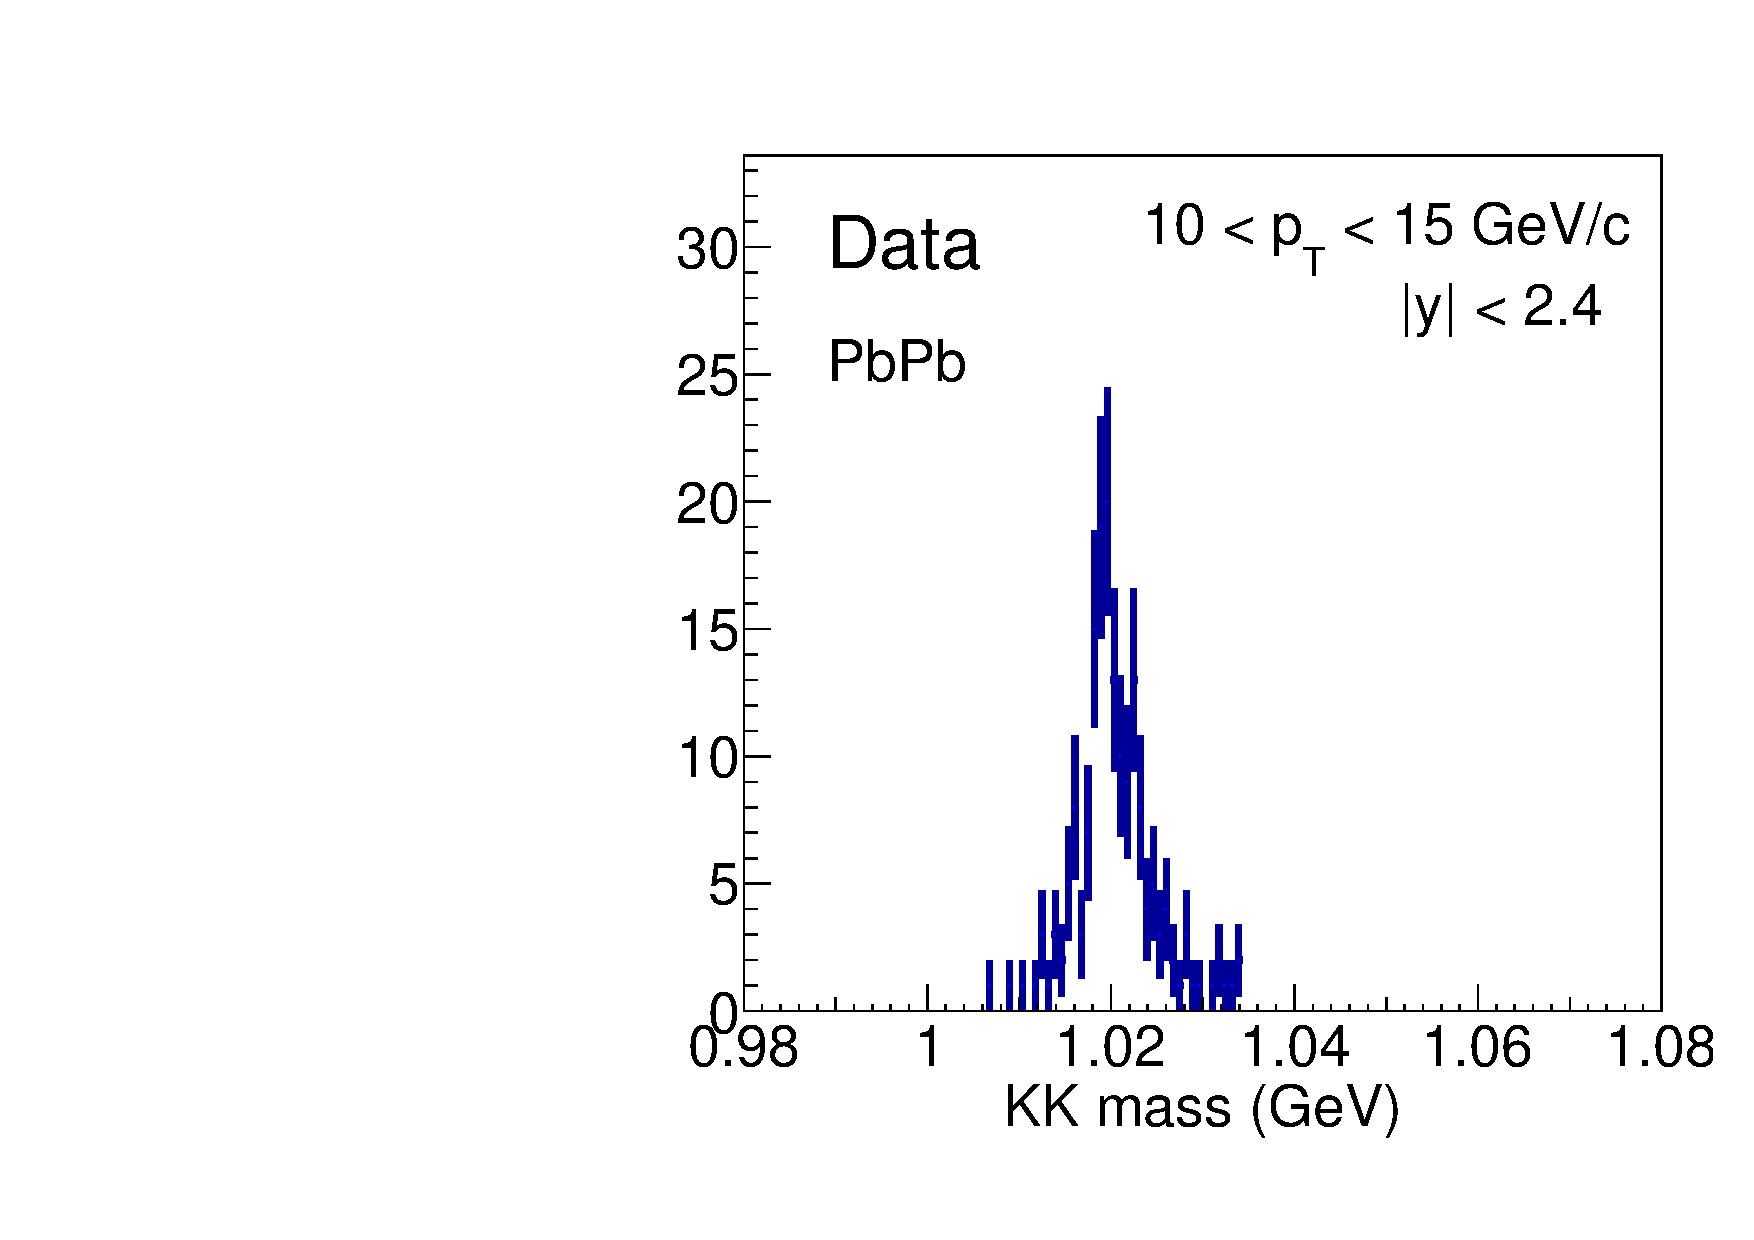
\includegraphics[width=0.42\textwidth]{Figures/Chapter4/data_PbPb_1_Btktkmass.pdf}
\caption{The $J/\psi$ (left) and $\phi$ (right) meson mass distributions after BDT selections for MC (top) and data (low) in PbPb analysis are shown above.}
\label{mesonpeakPbPb}
\end{center}
\end{figure}

We can see clear $J/\psi$ and $\phi$ peaks after apply the selections in both data and MC, which suggest that our selections are reasonable.


\section{B Mesons Candidates MC-Data Comparison}

Ideally, if the simulation is impeccable, the RECO distribution in the MC should match perfectly with data. Nevertheless, there is always limitation in the MC simulation because the incorrect model of physics processes in the generation side or poor model of detector conditions the in the reconstruction side. The discrepancy should be quantified as a source systematic uncertainties. 


\section{Background Studies} 


\section{Signal Extraction} 

\subsection{B-meson Invariant Mass Distributions}

\subsection{Fitting Models}

\subsection{Raw Yield Extraction}

\subsection{Signal Significance Estimation}


\section{Acceptance and Efficiency Correction} 

\subsection{Analysis Challenges}

\subsection{Fiducial Measurement}

\subsection{Fine 2D Efficiency Map}

\subsection{Data-Drive Efficiency Correction}

\subsection{Tag \& Probe Techniques}

\subsection{Nominal Results}

\section{Cross Section Results} 

\section{Validation Tests} 

\subsection{Mass Scraping Test}

\subsection{Raw Yield Closure}

\subsection{Efficiency Closure}

\subsection{sPlot Closure}


\section{Statistical Uncertainties Determination} 

\subsection{Data Bootstrapping}

\subsection{Statistical Uncertainties Interpretation}

\section{Systematic Uncertainties Estimation} 

\subsection{Global Observables}

\subsection{Branching Ratios}

\subsection{Tracking Efficiency}

\subsection{Muon Efficiency}

\subsection{Selection Efficiency}

\subsection{Signal Extraction}

\subsection{Summary}

\section{Final Results} 

\subsection{$B^0_s$ and $B^{+}$ Cross Section}

\subsection{$B^0_s/B^{+}$ Ratio}

\subsection{$B^0_s$ and $B^{+}$ Nuclear Modification Factor}

